% =====================================================================
%  THE ESCALATION TAX -- submission to Expert Systems with Applications
%
%  ANONYMISED MANUSCRIPT. ESWA reviews double-anonymised: no author names,
%  affiliations, e-mail addresses or acknowledgements may appear here or
%  in the supplementary material. They live on the separate title page
%  (title-page.tex); build_submission.py fails if any leaks in.
%
%  Compact rewrite of the IEEE Access draft in paper/. Material cut from
%  the manuscript is in supplementary-material.tex, submitted separately
%  and cited from the text.
%
%  Build: python build_submission.py (or pdflatex, bibtex, pdflatex x2)
% =====================================================================
\documentclass[final,5p,times,twocolumn]{elsarticle}

\usepackage{booktabs}
\usepackage{graphicx}
\usepackage{amsmath}
\usepackage{amssymb}
\usepackage{tabularx}
\usepackage{xurl}

\graphicspath{{figures/}}

\newcommand{\cells}{\mathcal{C}}
\newcommand{\cstar}{c^{*}}
\newcommand{\cost}{\mathrm{cost}}
\newcommand{\Tax}{\mathrm{Tax}}
\newcommand{\Esc}{\mathrm{Esc}}
\newcommand{\Stk}{\mathrm{Stk}}
\DeclareMathOperator*{\argmin}{arg\,min}
\DeclareMathOperator*{\argmax}{arg\,max}

\journal{Expert Systems with Applications}

\begin{document}

\begin{frontmatter}

\title{The escalation tax: measuring what manual model and reasoning-mode
selection costs, and whether a one-shot router recovers it}

\begin{abstract}
Tiered language-model services leave users to choose a model size and,
increasingly, whether the model should reason before answering. Users
misallocate in two directions: escalating after each failure, paying for
every discarded attempt, or leaving a heavyweight configuration selected and
overpaying on prompts that never needed it. We call the excess over the
cheapest configuration that would have succeeded the escalation tax and
split it into escalation and stickiness. We ask whether a small router in
front of eight Qwen3 configurations (0.6 to 8 billion parameters, thinking
on and off) can pick that minimum sufficient configuration before generation
net of its own tokens, latency and energy. Every prompt of a
stratified corpus runs through all eight on a laptop GPU with metered board
power. We compare classical, encoder and language-model routers against
manual escalation policies and a self-verifying cascade, and measure the tax
on two further pools: thirteen public models and six hosted configurations
with paid reasoning effort. Leaving the largest thinking configuration
selected pays 12.96 times the minimum sufficient energy and a frugal climb
0.89 times, at 3{,}612 and 946\,J per solved prompt against the oracle's
635\,J. Whether routers beat that climb depends on how a failed route is
recovered. Recovering at the largest configuration, the best router spends
1.30 times the climb's energy per solved prompt, though 64\% less than the
sticky default; recovering by climbing instead, routers match it and four
beat it. Where users miss wrong answers, the router answers 7.1 points more.
\end{abstract}

\begin{keyword}
energy efficiency \sep hybrid thinking \sep inference cost \sep
large language models \sep model routing \sep reasoning effort \sep
test-time compute
\end{keyword}

\end{frontmatter}

\section{Introduction}
\label{sec:introduction}

Anyone who uses a tiered language-model service makes an allocation decision
before typing a word. Providers sell families of models that trade
capability against price and latency, and a growing number also expose a
second control: whether, and how much, the model should reason before it
answers \cite{openai_reasoning,anthropic_effort,google_thinking}. Open-weight
families ship the same two axes; Qwen3 offers dense models from 0.6B to 14B
parameters with a switch between thinking and non-thinking modes and a
controllable thinking budget \cite{qwen3}. Reasoning traces raise accuracy on
hard problems \cite{wei2022cot,deepseek2025r1}, but they multiply the number
of generated tokens, and the choice of when to pay for them is left to the
person holding the keyboard.

People get that choice wrong in two opposite directions. The first is
under-provisioning: start with a small, cheap configuration, notice a wrong
answer, and move up. Every failed attempt is billed in full, and so is the
prompt, which has to be resent at each step. The second is
over-provisioning: a heavyweight configuration chosen for yesterday's hard
task stays selected, and today's trivial prompts pay its premium. Reasoning
models make the second failure worse because they tend to produce long traces
for questions that need none, a pattern the efficient-reasoning literature
calls overthinking \cite{sui2025stopoverthinking,alomrani2025reasoningbudget}.
Both failures waste tokens, time and energy, and neither has been measured
against the configuration that would have been sufficient.

Model routing is the obvious remedy, and there is a large literature on it
\cite{moslem2026routingsurvey}. Cascades query models in order of cost and
stop when a scorer accepts an answer \cite{chen2023frugalgpt,aggarwal2024automix}.
Predictive routers pick a model from the query alone
\cite{ding2024hybridllm,ong2024routellm}. More recent work routes over
reasoning mode \cite{zhang2025synapseroute,lee2026dart} and over model and
reasoning strategy jointly \cite{pan2026routetoreason}. These systems are
evaluated against static single-model policies, random assignment, an oracle,
or an automated cascade. None of the work we located evaluates them against
the policy people actually follow, which is manual escalation with the prompt
resent at every step. Energy-aware routers do measure power, but they route
over model choice or processing pipeline rather than reasoning mode, and they
report savings gross of the router's own consumption
\cite{ziller2026greenserv,li2026ecothink}. Routers that control reasoning
effort report tokens and latency, not joules \cite{lee2026dart}.

This paper studies one-shot selection of the \emph{minimum sufficient
configuration}: the cheapest cell of a model-size by reasoning-mode grid that
still answers a prompt correctly, predicted before any generation. We define
the \emph{escalation tax} as the cost a policy incurs beyond that
configuration, and split it into an escalation component, paid for attempts
that failed, and a stickiness component, paid for finishing on a
configuration more expensive than necessary. The study runs on hardware most
practitioners own: a laptop with an 8\,GB consumer GPU, where quantisation is
forced, one model fits in memory at a time, and every joule is measured from
board power rather than estimated from rated power.

The contributions are as follows.
\begin{itemize}
  \item A formal definition of the escalation tax and its decomposition, with
        a family of manual escalation policies evaluated under both perfect
        and imperfect failure detection (Section~\ref{sec:methodology}).
  \item An oracle-labelled corpus in which every prompt is run through all
        eight cells of a Qwen3 size-by-mode grid, recording per-cell success,
        token counts, latency and measured energy
        (Section~\ref{sec:setup}).
  \item A comparison of three router families---classical classifiers,
        fine-tuned encoders and a small language model used as a
        router---under \emph{net} accounting, in which each router's own
        tokens, latency and energy are subtracted from the saving it
        produces.
  \item A measured characterisation of the energy cost of the reasoning-mode
        axis, reported as joules per \emph{solved} query, so that a cheap
        configuration that fails and forces a retry is not flattered.
  \item The same tax measured on two pools the laptop cannot host: thirteen
        public models and six hosted cells in which reasoning effort is a
        paid setting (Section~\ref{sec:results}).
\end{itemize}

The tax is large, and most of it comes from where a user stays rather than
how they climb. Leaving the 8B thinking cell selected pays 12.96 times the
minimum sufficient energy and answers 79.8\% of prompts; a frugal climb with
thinking off pays 0.89 times and answers 92.2\%. On gradable tasks, moving up
a size below 8B without thinking answers more prompts than turning thinking
on, for 3.8 to 5.5 times less energy per solved prompt; on open-ended
requests, graded by a model judge that agrees with a human only moderately,
thinking is far cheaper, yet the frugal climb still pays the least tax. How a
router compares with that climb turns on how a failed route is recovered.
Sent to the largest cell, the best router spends 1.30 times the climb's
energy per solved prompt, though 64\% less than the sticky default;
recovering by climbing from the routed cell instead, every router comes
within 6\% of the climb and four are cheaper than it. Detection matters as
much: when users accept 15\% of wrong answers, the router answers 7.1 points
more than the climb, because it makes fewer attempts at which to be fooled.

Section~\ref{sec:related} reviews the three literatures the problem sits
between, Section~\ref{sec:methodology} formalises the tax and the routers,
Section~\ref{sec:setup} gives the setup, and
Sections~\ref{sec:results} to \ref{sec:conclusion} present, interpret and
conclude from the results.

\section{Related work}
\label{sec:related}

The problem sits where three bodies of work meet: routing and cascading
across models, control of reasoning effort at inference time, and
measurement of the energy inference consumes. Table~S1 of the supplementary
material places the closest systems side by side.

\subsection{Routing and cascading across models}
\label{sec:related-routing}

This paper is concerned with routing that sends whole queries to separate
models, each of which could answer alone, rather than with routing tokens
between expert sub-networks inside one model. Moslem and Kelleher survey that
literature and divide it into routing, which commits before generation, and
cascading, which tries models in sequence \cite{moslem2026routingsurvey}.

\emph{Cascades.} FrugalGPT sends a query through models of increasing price
and stops when a learned scorer accepts the answer, reporting up to 98\%
lower cost than the best individual model \cite{chen2023frugalgpt}. AutoMix
replaces the external scorer with few-shot self-verification by the small
model and decides whether to escalate with a partially observable Markov
decision process, reporting cost reductions above 50\%
\cite{aggarwal2024automix}. AutoMix is the closest published idea to the
question asked here, because it treats escalation as a sequential decision;
its decision state, however, is the model's confidence in its own answer
rather than the cost already spent, and it is an automated policy rather than
a model of what a user does. Both cascades share a structural cost: the cheap
model must generate before the system can decide, so every escalated query
pays for at least one discarded answer.

\emph{Predictive routers.} Hybrid LLM estimates from the query alone whether
a small model's answer will match a large model's, and exposes a threshold
that trades quality for cost, reporting 40\% fewer large-model calls at no
loss in quality \cite{ding2024hybridllm}. RouteLLM learns a strong-versus-weak
decision from human preference data and reports more than a twofold cost
reduction \cite{ong2024routellm}. Later work trains a query encoder
with dual contrastive losses \cite{chen2024routerdc}, routes to models unseen
during training with an excess-risk bound \cite{jitkrittum2025universal},
aligns a router with user-defined preferences so models can be added without
retraining \cite{tran2025archrouter}, and interleaves a router's own
deliberation with calls to other models over several rounds
\cite{zhang2025routerr1}. Published benchmarks make routers comparable, among
them LLMRouterBench, whose released outcomes and prices this study reuses
\cite{li2026llmrouterbench}. Across this work, cost is denominated in API
price, model calls or tokens, and the comparison points are static, random,
oracle or automated policies.

\subsection{Reasoning effort and test-time compute}
\label{sec:related-reasoning}

Chain-of-thought prompting improves multi-step reasoning by spending
generated tokens on intermediate steps \cite{wei2022cot}, reinforcement
learning now trains models that produce long traces unprompted
\cite{deepseek2025r1}, and Qwen3 builds the control into the model, serving
thinking and non-thinking behaviour from one set of weights \cite{qwen3}.
Long traces are not always useful: Sui
et al.\ document reasoning models spending many tokens on easy questions
\cite{sui2025stopoverthinking}, and Alomrani et al.\ organise adaptive
test-time compute into controllability under a fixed budget and adaptiveness,
where the budget depends on the input \cite{alomrani2025reasoningbudget}.
Selecting a reasoning mode per prompt is an instance of the second tier.

A recent group of papers routes over whether and how much to think, usually
within one model. SynapseRoute sends medical questions to the thinking or
non-thinking mode of a dual-state model, reporting 36.8\% lower inference
time and that about 58\% of its questions need no reasoning
\cite{zhang2025synapseroute}. A lightweight router head can make the same
choice for ranking tasks \cite{guo2026thinkwhenneeded}, while DART is
training-free, reading difficulty from the agreement of two cheap drafts and
cutting thinking tokens by 32--73\% \cite{lee2026dart}. Learning
When to Think moves the decision inside the model, which emits NoThink, Short
or Long as its first token \cite{kassenaar2026learningwhentothink}, and
HRBench finds that the preferred switching strategy depends on model scale
and task domain \cite{ning2026hrbench}. Route to Reason is the closest prior
work to the grid studied here, selecting jointly among seven models and four
reasoning strategies under a budget constraint \cite{pan2026routetoreason};
joint selection of model and reasoning effort is therefore not, by itself, a
new idea, and we do not claim it as one.

All of this work depends on an assumption that is rarely tested: that a
model's thinking and non-thinking modes are genuinely different operating
points. Wang et al.\ found only partial separation in hybrid-thinking models,
with reasoning behaviour leaking into non-thinking outputs
\cite{wang2025demystifying}, which is why we test separation on our own
checkpoints before labelling (Section~\ref{sec:setup-gates}).

\subsection{Energy, carbon and energy-aware routing}
\label{sec:related-energy}

Strubell et al.\ brought the cost of training to the field's attention
\cite{strubell2019energy} and Schwartz et al.\ argued for efficiency as a
first-class result \cite{schwartz2020greenai}. Lacoste et al.\ convert
compute into emissions with regional grid intensity
\cite{lacoste2019quantifying}, and Patterson et al.\ show how strongly
training emissions depend on hardware and location \cite{patterson2021carbon}.
For inference, Luccioni et al.\ measured energy and carbon per 1{,}000
queries across task types and found wide variation
\cite{luccioni2024powerhungry}. Tuning GPU frequency and batch size
\cite{xu2025camel} or managing key--value cache memory \cite{kwon2023vllm}
makes each configuration cheaper to run without deciding which to run, and is
therefore orthogonal to routing.

Three routers treat energy or latency as part of the objective. GreenServ
routes among 16 open models, measures GPU energy on an A100 and reports a
31\% energy reduction with 22\% higher accuracy than random routing, but does
not subtract the router's own energy \cite{ziller2026greenserv}. EcoThink
sends each query to a retrieval or a reasoning path with a distilled
classifier and reports a 40.4\% energy reduction and 1.32\,gCO$_2$e per query
against 4.52 for GPT-4o, with energy partly estimated from thermal design
power and the router uncharged \cite{li2026ecothink}. Yang et al.\ route
among edge experts on RTX~4090 GPUs, optimising quality of service and
latency without measuring energy \cite{yang2025qosrouting}. Energy-aware
routing and carbon reporting are therefore established, and neither is a
contribution of this paper; what is missing is a router over reasoning mode
whose own measured energy is netted out.

Open-ended prompts cannot be graded by string match, so studies that include
them rely on model judges. Zheng et al.\ found a strong judge agreeing with
human preferences about as often as humans agree with each other, while
documenting position, verbosity and self-enhancement biases
\cite{zheng2023judging}. Those biases motivate the out-of-family judge and
two-sided validation of Section~\ref{sec:setup-judge}.

\subsection{Positioning}
\label{sec:related-gap}

Four questions remain open in the literature we located. First, the
escalation tax is unmeasured: no study formalises manual escalation, in which
each failed attempt is billed in full and the prompt is resent. Second,
router energy is not netted out; we found no study that subtracts the
selector's own measured energy, or asks when a language-model router stops
paying for itself against a linear classifier. Third, the reasoning-mode axis
has no measured energy cost: routers over reasoning mode report tokens and
latency, and routers that measure energy do not route over mode. Fourth,
energy is not normalised by success; energy per \emph{solved} query, which
charges a cheap failure for the retry it causes, was not found.

\section{Methodology}
\label{sec:methodology}

\subsection{Configuration grid and cost}
\label{sec:grid}

The routed pool is a grid, not a ladder: four model sizes crossed with two
reasoning modes, giving eight cells $\cells = \{c_1, \dots, c_8\}$
(Table~\ref{tab:grid}). All cells come from one family, Qwen3, which offers a
size ladder in which every model runs with or without a thinking phase
\cite{qwen3}, so that size and mode are the only things that vary between
cells: tokenizer, training recipe and chat template stay the same.
Quantisation is held fixed at 4-bit (Q4\_K\_M) for the same reason, at the
cost of describing quantised models only.

\begin{table}[ht]
\centering
\caption{The eight-cell configuration grid. Sizes on disk are for the
Q4\_K\_M weights used in all experiments.}
\label{tab:grid}
\begin{tabular}{@{}cllr@{}}
\toprule
Cell & Model & Mode & Weights \\
\midrule
$c_1$ & Qwen3-0.6B & no-think & 0.52\,GB \\
$c_2$ & Qwen3-0.6B & think    & 0.52\,GB \\
$c_3$ & Qwen3-1.7B & no-think & 1.36\,GB \\
$c_4$ & Qwen3-1.7B & think    & 1.36\,GB \\
$c_5$ & Qwen3-4B   & no-think & 2.62\,GB \\
$c_6$ & Qwen3-4B   & think    & 2.62\,GB \\
$c_7$ & Qwen3-8B   & no-think & 5.23\,GB \\
$c_8$ & Qwen3-8B   & think    & 5.23\,GB \\
\bottomrule
\end{tabular}
\end{table}

We do not assume the cells are ordered by parameter count: a thinking cell of
one size can cost more than a non-thinking cell of the next size up, and
whether it does depends on the prompt. Cost is therefore measured per prompt
$q$ and per cell $c$, in three units,
\begin{align}
  \cost_{\mathrm{tok}}(c, q) &= \alpha\, n_{\mathrm{in}}(c, q)
                              + \beta\, n_{\mathrm{out}}(c, q),
  \label{eq:tokcost}\\
  \cost_{\mathrm{lat}}(c, q) &= \text{wall-clock time of the request (s)},
  \label{eq:latcost}\\
  \cost_{\mathrm{E}}(c, q)   &= \text{GPU energy of the request (J)},
  \label{eq:energycost}
\end{align}
where $n_{\mathrm{in}}$ and $n_{\mathrm{out}}$ are input and generated token
counts, the latter including any reasoning trace, and $\alpha$ and $\beta$
are per-token prices that make the token cost comparable with metered API
billing. Energy is measured, not estimated (Section~\ref{sec:energy}). All
definitions below apply to any unit; we write $\cost(c, q)$ when the unit
does not matter.

\subsection{Minimum sufficient configuration and the escalation tax}
\label{sec:tax}

Let $s(q, c) \in \{0, 1\}$ indicate whether cell $c$ produces an acceptable
answer to $q$ under the criteria of Section~\ref{sec:setup-labels}. The
\emph{minimum sufficient configuration} is the cheapest cell that succeeds,
\begin{equation}
  \cstar(q) = \argmin_{c \in \cells \,:\, s(q, c) = 1} \cost(c, q).
  \label{eq:cstar}
\end{equation}
It is undefined when no cell succeeds; those prompts are kept and reported as
the \emph{unservable fraction}, since dropping them would flatter every
policy, which pays to find out that they cannot be served.

A manual escalation policy $\pi$ consists of a starting cell and an ordered
ladder of cells to try next. The user submits $q$ to the starting cell; when
an answer is judged a failure, the \emph{whole prompt} is resubmitted to the
next rung, until an answer is accepted or the ladder runs out. With
$a_1, \dots, a_m$ the cells attempted and $a_m$ the one finally accepted, the
policy's cost is
\begin{equation}
  \mathrm{Cost}(\pi, q) = \sum\nolimits_{j=1}^{m} \cost(a_j, q).
  \label{eq:policycost}
\end{equation}
Because $n_{\mathrm{in}}$ enters \eqref{eq:tokcost} at every attempt, a long
prompt makes escalation expensive even when each failed answer is short; that
resubmission cost is absent from cascade evaluations charging only for
generated tokens. The escalation tax is the excess over the minimum
sufficient configuration,
\begin{equation}
  \Tax(\pi, q) = \mathrm{Cost}(\pi, q) - \cost\bigl(\cstar(q), q\bigr),
  \label{eq:tax}
\end{equation}
and splitting \eqref{eq:policycost} at the final attempt gives an exact
decomposition into two terms with different causes,
\begin{align}
  \Tax(\pi, q) &= \Esc(\pi, q) + \Stk(\pi, q), \label{eq:decomp}\\
  \Esc(\pi, q) &= \sum\nolimits_{j=1}^{m-1} \cost(a_j, q), \nonumber\\
  \Stk(\pi, q) &= \cost(a_m, q) - \cost\bigl(\cstar(q), q\bigr). \nonumber
\end{align}
\emph{Escalation} is the cost of attempts thrown away; \emph{stickiness} is
what the user overpays for the configuration that finally answered. When
failures are always detected, $a_m$ succeeded, so by \eqref{eq:cstar} both
components are non-negative. A user who begins on the largest thinking cell
and never moves pays only stickiness; one who climbs from the smallest cell
and stops exactly at $\cstar(q)$ pays only escalation. Most trajectories pay
some of each, and the two respond to different remedies, which is why we
report them separately.

\begin{table*}[ht]
\centering
\caption{Manual escalation policies. Cells as in Table~\ref{tab:grid}.}
\label{tab:policies}
\begin{tabularx}{\textwidth}{@{}l p{3.4cm} >{\raggedright\arraybackslash}X@{}}
\toprule
Policy & Ladder & Behaviour modelled \\
\midrule
P1 & $c_1{\to}c_3{\to}c_5{\to}c_7{\to}c_8$ & \emph{Frugal climb}: cost-conscious; larger model first, thinking last \\
P2 & $c_1{\to}c_2{\to}c_4{\to}c_6{\to}c_8$ & \emph{Think first}: turns on thinking before moving up a size \\
P3 & $c_8$ only & \emph{Sticky high}: heavyweight left selected from earlier work \\
P4 & Start drawn from an assumed distribution over cells, then the P1 ladder & \emph{Sticky mixed}: a population of users \\
\bottomrule
\end{tabularx}
\end{table*}

We construct the comparator ourselves, so we construct it generously.
Table~\ref{tab:policies} lists four policies ranging from frugal to wasteful.
P4 models a population of users who start wherever they left off; having no
usage logs, its starting distribution is an assumption, uniform over the
eight cells in the primary analysis and, as a sensitivity analysis, a
distribution in which half of all queries start at $c_8$. Both are labelled
as assumed wherever reported.

An escalating user must notice that an answer is wrong. Under \emph{oracle
detection} the user always notices and never discards a correct answer; this
regime gives the manual policies their highest solved rate and is the one we
quote in headline results. It does not bound their cost in either direction,
since rejecting a right answer adds attempts while accepting a wrong one ends
a climb early. Under \emph{imperfect detection} the user accepts a wrong
answer with probability $p_{\mathrm{acc}}$ and rejects a correct one with
probability $p_{\mathrm{rej}}$, and the last rung's answer is kept whatever
its quality. A prompt may then end unsolved, so costs are also reported per
\emph{solved} prompt,
\begin{equation}
  \bar{\cost}_{\mathrm{solved}}(\pi) =
  \frac{\mathbb{E}_q\bigl[\mathrm{Cost}(\pi, q)\bigr]}
       {\Pr_q\bigl[\text{$q$ solved under $\pi$}\bigr]}.
  \label{eq:persolved}
\end{equation}
Having no measurement of the two probabilities, we sweep them:
$p_{\mathrm{acc}} \in \{0, 0.05, 0.10, 0.15, 0.20, 0.30\}$ and
$p_{\mathrm{rej}} \in \{0, 0.05, 0.10\}$, and show
$p_{\mathrm{acc}} = 0.15$, $p_{\mathrm{rej}} = 0.05$ as an illustration.
Every outcome, including the tax and the probability of solving a prompt, is
an expectation over the user's accept-or-reject decisions, computed exactly
from the labelled success vectors rather than by simulating users.

\subsection{Routers as per-cell success predictors}
\label{sec:routers}

Every router predicts a vector of success probabilities, one per cell, rather
than a single class label,
\begin{equation}
  f(q) = \bigl(\hat{p}_1(q), \dots, \hat{p}_8(q)\bigr), \qquad
  \hat{p}_i(q) \approx \Pr\bigl[s(q, c_i) = 1\bigr],
  \label{eq:router}
\end{equation}
and a separate rule turns the vector into a decision. Given a quality
threshold $\tau \in [0, 1]$, the router picks the cheapest cell it believes
will succeed,
\begin{equation}
  \hat{c}_\tau(q) =
  \begin{cases}
    \displaystyle\argmin_{i \,:\, \hat{p}_i(q) \geq \tau} \bar{\cost}(c_i)
      & \text{if some } \hat{p}_i(q) \geq \tau,\\[1.2ex]
    \displaystyle\argmax_{i} \hat{p}_i(q) & \text{otherwise},
  \end{cases}
  \label{eq:selection}
\end{equation}
where $\bar{\cost}(c_i)$ is cell $c_i$'s mean cost on the training split,
because the true per-prompt cost is unknown before generation. Separating
prediction from decision yields a whole cost--quality curve from one trained
router by sweeping $\tau$, as Hybrid LLM exposes a quality knob at test time
\cite{ding2024hybridllm}, and lets the asymmetry between the two kinds of
error be handled by moving $\tau$ instead of retraining: routing one cell too
low produces a failure and a retry, while routing one cell too high only
wastes compute. Direct eight-way classification of $\cstar(q)$ is kept as an
ablation.

A router that picks a failing cell does not end the interaction. We charge a
routed policy as we charge a manual one: the routed cell is the first
attempt, and on failure the prompt is resubmitted once to the largest
thinking cell $c_8$. As a sensitivity analysis, a failed routed attempt
instead continues up the P1 ladder from the routed cell. The tax is then
computed with \eqref{eq:tax} exactly as for $\pi$. For each cost unit,
recovery rule and detection regime, $\tau$ is chosen on the validation split
to minimise net cost per solved prompt, router cost included, and the test
split is evaluated once at that value.

Three router families span four orders of magnitude in their own cost.
\emph{R1, classical classifiers:} logistic regression on TF-IDF word and
character $n$-grams; gradient-boosted trees
\cite{chen2016xgboost,ke2017lightgbm} on hand-built features (prompt length,
digit and operator density, code fences, question type, readability); and
logistic regression on frozen Sentence-BERT embeddings
\cite{reimers2019sbert} from all-MiniLM-L6-v2. All run
on a CPU. \emph{R2, fine-tuned encoders:} DistilBERT \cite{sanh2019distilbert}
and DeBERTa-v3-small \cite{he2023debertav3}, fine-tuned end to
end with eight sigmoid outputs, with class-weighted binary cross-entropy so
that success and failure carry equal weight in each cell. \emph{R3, a
language model as router:} Qwen3-0.6B, the smallest pool member, is shown the
eight configurations labelled A to H and asked which is the cheapest that
will answer correctly, prompted zero-shot and few-shot. Rather than decode a
letter, we read the next-token distribution at the first answer token, keep
the mass on the eight letters and renormalise, which constrains the answer to
a valid configuration and yields a distribution over $\cstar(q)$; treating
success as monotone in mean cost, $\hat{p}_i(q)$ in \eqref{eq:router} is the
mass on configurations whose mean cost does not exceed that of $c_i$. A third
variant adds LoRA adapters \cite{hu2022lora} trained to name the $\cstar$ of
each training prompt. A router larger than the models it routes between
defeats its own purpose, so we deliberately use the smallest pool member.
Because misrouting costs are asymmetric, a cost-sensitive variant of each R1
and R2 router weights errors by their realised cost consequence.

\subsection{Net-of-router accounting and the cascade baseline}
\label{sec:net}

A router is itself a workload. Each router's latency and energy per decision
are measured with the same instruments as the pool and added to the cost of
every query it routes, so that for a router $r$ and baseline policy $b$ the
\emph{net saving} is
\begin{equation}
  S_{\mathrm{net}}(r; b) =
    \mathbb{E}_q\bigl[\mathrm{Cost}(b, q)\bigr]
  - \mathbb{E}_q\bigl[\mathrm{Cost}(r, q) + \cost_{\mathrm{route}}(r, q)\bigr].
  \label{eq:netsaving}
\end{equation}
In token cost the extra term is non-zero only for R3, which consumes tokens
of its own; its decisions run through the labelling harness as short
generations and are metered per prompt exactly as the pool's are. The LoRA
variant is charged the zero-shot probe's metered cost, an upper bound, since
the probe decodes up to eight tokens where the variant needs one forward
pass. R1 and R2 decide on the CPU, which NVML cannot see, so their energy per
decision is bounded above by decision time multiplied by the upper end of the
processor's configurable power range (54\,W), and that bound is charged.

The strongest published alternative to predicting in advance is to try the
cheap configuration and check. We implement a cascade in the style of AutoMix
\cite{aggarwal2024automix}: generate on the cheapest cell, ask the same model
to verify its answer with a few-shot prompt whose four worked examples are
generic, and escalate along the P1 ladder when verification fails. The
verifier's confidence is read from a single forward pass as
$P(\text{Yes})/\bigl(P(\text{Yes}) + P(\text{No})\bigr)$ at its first answer
token, and a query escalates when that confidence falls below a threshold
chosen on the validation split, as $\tau$ is for a router. The answer from
$c_8$ is kept without verification, and AutoMix's POMDP meta-verifier is
omitted, which may weaken the cascade relative to the original method.
Verification calls are metered and charged like any other generation. This
baseline pays for failed attempts as a user does, but decides with
information from the answer itself, so beating it requires that predicting
before generation save more than that information is worth.

\subsection{Energy measurement}
\label{sec:energy}

GPU board power is read through NVIDIA's management library, NVML
\cite{nvidia_nvml}, by a sampling thread polling instantaneous power every
100\,ms. Two properties of the hardware shape the method, both established by
the telemetry gate of Section~\ref{sec:setup-gates}: the cumulative energy
counter NVML also exposes is unusable on this GPU, so energy is always
integrated from sampled power; and reported power refreshes only every 0.5\,s
and is smoothed, so a short answer from the smallest model can finish inside
one refresh period and its energy cannot be read from its own time window.

Energy is therefore integrated over \emph{batch windows}. Prompts are taken
in batches of 20, and each batch is run twice back to back on the loaded
model, once per mode, so every window holds a single cell; which mode runs
first alternates between batches. Each window is extended by a 6\,s tail after
its last generation, because reported power takes about 5\,s to decay once
generation stops, and the integral is computed with the trapezoidal rule.
Readings above 200\,W, which the GPU cannot draw under its 115\,W limit, are
discarded as read errors. We report board energy, the raw integral, and
dynamic energy, which subtracts the idle power of the GPU with the model
loaded, measured over 60\,s after warm-up and 30\,s at the end of each
session; dynamic energy is what we attribute to queries. Each query receives
a share of its window's dynamic energy in proportion to its share of the
window's generation wall time, with token share as a check. A window is
discarded and rerun, up to four times, if utilisation at the end of its tail
shows another workload or if any generation reloaded the model. Routers that
run on the GPU are measured the same way.

Two derived measures connect energy to the tax. \emph{Joules per solved
query} divides the energy a policy spends, failed attempts included, by the
number of prompts it solves, so a cheap configuration that fails and triggers
a retry is charged for the retry. \emph{Carbon} is reported as
$\mathrm{gCO_2e} = (E/3.6 \times 10^{6})\,I$ for a grid intensity $I$ in
gCO$_2$e/kWh, following Lacoste et al.\ \cite{lacoste2019quantifying} and
Luccioni et al.\ \cite{luccioni2024powerhungry}. The intensity belongs to the
grid rather than the experiment, and grids differ by more than an order of
magnitude, so carbon is reported across a bracket of intensities; the
conversion is linear, so any figure rescales.

\section{Experimental setup}
\label{sec:setup}

\subsection{Hardware, software and decoding}
\label{sec:setup-hardware}

All local experiments run on one laptop: an AMD Ryzen~7 8845HS CPU with
16\,GB of system memory and an NVIDIA GeForce RTX~4060 Laptop GPU with 8\,GB
of memory, driver 616.56 and an enforced board power limit of 115\,W. The
driver was updated to 616.92 between the main labelling run and the later
stages; the noise stage, which resamples prompts and cells the main run
measured, shows energy per output token under 616.92 at 0.89 to 1.01 times
that under 616.56. Every cell of the grid was measured under 616.56, so no
comparison between cells crosses the change. Models are served by Ollama \cite{ollama} from GGUF
weights quantised to Q4\_K\_M \cite{gerganov2023llamacpp}. Each model is
addressed by an explicit quantisation tag, and its weight digest, parameter
count, context length and chat template are recorded in a manifest before any
generation, so a silently updated tag cannot change the models between runs.

The 8\,GB memory limit means one model is loaded at a time, so runs are
organised \emph{model-major}: each model is loaded once, all prompts run in
both modes, and the model is unloaded before the next. Within a model,
prompts are processed in batches of 20, each batch running its two modes as
separate measurement windows with the leading mode alternating, so that slow
drift in temperature or background load cannot line up with one mode. The
harness waits for 30\,s of continuous GPU idleness before loading a model or
repeating a window, and checks that the whole model is placed on the GPU.

Greedy decoding is discouraged for Qwen3's thinking mode, so each mode uses
its recommended sampling settings \cite{qwen2025modelcard}: temperature 0.6,
top-$p$ 0.95 and top-$k$ 20 for thinking, and 0.7, 0.8 and 20 for
non-thinking. Every generation receives its own seed, derived
deterministically from the prompt, cell, sample index and run variant, and
stored with the output. The labelling runs draw one sample per prompt and
cell ($k = 1$), so a noise subset of 25 prompts per family receives two
further samples in every cell to measure how often a label would change on
resampling; three samples throughout were the original plan, but one sample
across the eight cells takes about 112\,s per prompt, and tripling that would
have tripled a run that already takes days.

Generation length is capped, and an answer that hits the cap counts as a
failure, because a truncated answer is of no use in deployment: 4{,}096 new
tokens in thinking mode, trace included, and 2{,}048 without. The caps matter
more than we expected, so their effect is measured rather than assumed. A
sample of capped generations, up to 40 per size and mode and spread evenly
over families, is rerun with an 8{,}192-token cap and a 10{,}240-token
context (9{,}216 at 8B, where the larger context no longer fits in GPU
memory), and we report how often the longer cap turns a failure into a
success and how often that moves $\cstar(q)$. Each server session runs one
thinking and one non-thinking warm-up generation, which are discarded.

\subsection{Corpus, labelling and grading}
\label{sec:setup-labels}

The corpus covers four task families of 400 prompts each. Three are graded
programmatically: mathematics, from GSM8K \cite{cobbe2021gsm8k} (200) and
MATH-500 \cite{hendrycks2021math,lightman2024verify} (200); code, from
HumanEval \cite{chen2021humaneval} (154) and MBPP \cite{austin2021mbpp} (246);
and multiple choice, from MMLU \cite{hendrycks2021mmlu} (200) and
ARC-Challenge \cite{clark2018arc} (200). The fourth, open-ended requests from
Dolly-15k \cite{conover2023dolly} (400), is the traffic that motivates the
problem and needs a judge (Section~\ref{sec:setup-judge}).

Prompts are drawn with a fixed, recorded seed. Each source is walked in
round-robin order over strata of an a-priori difficulty proxy where one
exists---MATH level, MMLU subject and MBPP task band---so that any prefix of
the order is balanced across strata; a 100-prompt pilot per family is
therefore nested in the full corpus, and its first 25 prompts form the noise
subset. Near-duplicates are removed by hashing normalised prompt text across
sources as well as within them, and prompts longer than 2{,}048 tokens are
excluded so that context length does not vary with the size axis.

Every prompt is run through all eight cells, recording the full success
vector $s(q, c_1), \dots, s(q, c_8)$ with the token counts, latency and
energy of every cell. Routers are trained on that vector, which carries more
information than $\cstar(q)$ and is what allows $\tau$ to be swept at test
time. Success is decided per family: for mathematics the final answer is
extracted and normalised before comparison with the reference; for code the
generated function is executed against the dataset's unit tests in a
subprocess with a timeout and no network access, and succeeds only if every
test passes; for multiple choice the chosen option is parsed, and an
unparseable answer is a failure rather than a reason to resample. After
labelling, the corpus is split 60/20/20 into training, validation and test
sets by prompt, stratified by family and by $\cstar(q)$ computed in tokens,
so that every cost unit is evaluated on the same split; the test split is
used once, at the end.

\subsection{Judging open-ended answers}
\label{sec:setup-judge}

A judge drawn from the routed pool would grade its own family, so the judge
is Llama~3.1 8B Instruct \cite{grattafiori2024llama3} at Q4\_K\_M, run only
after labelling has finished. It sees the request, the human-written Dolly
response as a reference and the visible answer, and scores the answer from 1
to 5 on a fixed rubric, with 4 or more a success; for open requests such as
brainstorming the rubric treats the reference as one acceptable answer among
many. Answers are scored one at a time in a seeded random order, to limit the
position and verbosity biases documented for model judges
\cite{zheng2023judging}, with greedy decoding constrained to a JSON reply.

The judge is validated from two sides before its labels are used. About 200
judged answers, stratified by category and verdict, are re-scored with the
same rubric by \texttt{gpt-5-mini} through a hosted API, a reference above
the local judge in capability and outside its family; and the first author
scores about 100 of them blind to model, mode and judge score. Agreement is
Cohen's $\kappa$ \cite{cohen1960kappa} on the success decision and
quadratic-weighted $\kappa$ \cite{cohen1968weighted} on the scores. The rule
for using the labels was fixed before any judge output existed: at
$\kappa \geq 0.60$ the open-ended family is reported with the others; from
0.40 to 0.60 it carries an explicit caveat; below 0.40 it moves to a
secondary analysis, these being the conventional boundaries of moderate and
substantial agreement \cite{landis1977measurement}. The judge scored all
3{,}583 eligible answers, reaching $\kappa = 0.42$ [0.23, 0.59] against the
first author's blind scores and 0.40 [0.27, 0.52] against
\texttt{gpt-5-mini}, which agrees with the first author at 0.74 [0.60, 0.86].
The family therefore carries the caveat and is reported separately.

\subsection{Baselines, metrics and statistics}
\label{sec:setup-stats}

Routers are compared with the eight static policies that always use one cell,
uniform random assignment, the oracle that always picks $\cstar(q)$, the four
manual policies of Table~\ref{tab:policies} under both detection regimes, and
the cascade of Section~\ref{sec:net}. We report cost--quality frontiers and
the normalised area beneath them, the tax and its components from
\eqref{eq:decomp}, net savings from \eqref{eq:netsaving}, cost per solved
query in each unit, the over- and under-routing rates with their separate
cost consequences, and router overhead per decision.

Every headline figure carries a 95\% percentile bootstrap confidence interval
from 10{,}000 resamples over prompts \cite{efron1993bootstrap}. All policies
and routers evaluated on the same prompts share one matrix of resampled
indices, so every comparison is paired by prompt and its interval is taken
over resampled differences. Two-sided $p$-values are obtained by inverting
the percentile interval, and the Holm--Bonferroni procedure
\cite{holm1979simple} corrects within each family of comparisons that asks
one question at a fixed cost unit, recovery rule and detection regime. For
routers, $\tau$ is fixed on the validation split before the test split is
resampled, so the intervals exclude the uncertainty of that choice. Each
trainable router is trained with three seeds, with intervals reported for the
first and the spread across seeds beside them.

\subsection{Validation gates}
\label{sec:setup-gates}

Two assumptions were tested before any labelling, and both gates are reported
in full in the supplementary material (Tables S2 and S3).

\emph{Gate 1, power telemetry.} NVML does not expose board power on every
laptop GPU. Recording 10\,s of idle, 8\,s of half-precision matrix
multiplication at about 90\% utilisation and 8\,s of cool-down, sampled power
behaved as expected: low at idle, following the step load within about a
second, and never exceeding the enforced limit. The cumulative energy counter
did not. It is reported as supported and increases monotonically, so a
routine check accepts it, yet the power it implies is 88\,W with the GPU
idle, 128\,W under load, above the enforced limit, and 257\,W during
cool-down, higher than under load. A units error would scale all three
windows by one factor and keep their order; these values do not follow real
power draw at all. We therefore integrate sampled power only, and the lesson
for other studies on laptop GPUs is that a supported, monotonic counter
should still be cross-checked against sampled power and the enforced limit.

\emph{Gate 2, separation of thinking modes.} The grid assumes a model's two
modes are different operating points, which Wang et al.\ found only partly
true of hybrid-thinking models \cite{wang2025demystifying}. On 60 prompts per
size, run once per mode under a common 4{,}096-token cap, three criteria
fixed in advance were all met at all four sizes: an area under the ROC curve
of at least 0.90 for thinking outputs being longer (observed 0.928 to 0.964),
at most 5\% of non-thinking responses containing a thinking trace or tag
(observed zero), and reasoning-marker density in non-thinking answers no more
than half that in thinking traces (observed 3--5\%). Marker counting is a
lexical proxy, and 60 prompts per size cannot rule out leakage on task types
we did not sample. The gate also showed that thinking dominates the compute
budget, taking 88\% of the time of one sample across the eight cells, and
that between 21\% and 32\% of thinking responses hit the cap, which is why
the cap-sensitivity reruns of Section~\ref{sec:setup-hardware} are part of
the design.

\subsection{Public-benchmark and hosted-frontier arms}
\label{sec:setup-arms}

The local pool stops at 8B parameters, so two further arms test whether the
analysis carries beyond it. The first applies the same policy and tax
computations, without local inference, to the published per-model outcomes
and costs of LLMRouterBench \cite{li2026llmrouterbench}, whose records store a
score, prompt and completion token counts and the provider's dollar charge
for one model on one query---which is what the resubmission term needs, since
a re-asked query pays its prompt tokens again at the stronger model's price.
We take the thirteen models of its performance--cost setting and the nine
datasets every one of them was run on, keeping per dataset the largest subset
all thirteen share, which leaves 12{,}168 queries. A pool of thirteen models
has no natural order, so the ladder is the cost--accuracy frontier in cost
order, whose top rung plays the part $c_8$ plays locally; P2 has no analogue
without a mode axis, and the thinking and non-thinking releases of
Qwen3-235B-A22B are compared separately in its place. Because the frontier is
a subset of the pool, a policy climbing it can fail on a query some
off-ladder model answers, so the tax is read alongside the success rate.
Intervals here use 2{,}000 resamples, the prompt set being ten times the
local corpus.

The second arm restores the mode axis at frontier scale. Three hosted models,
\texttt{gpt-5-nano}, \texttt{gpt-5-mini} and \texttt{gpt-5}, are crossed with
two reasoning efforts, \texttt{minimal} and \texttt{high}, giving six cells
$h_1 \dots h_6$ indexed as $c_1 \dots c_8$ are, priced at list prices
published on 12 September 2026 and halved by the batch discount. Prompts come
from those the local grid has already labelled, so every hosted $\cstar$ is
paired with a local one. Each request carries exactly the prompt text the
local pool saw, and the output caps mirror the local protocol; on a reasoning
model the cap counts reasoning tokens, so a truncated response is a failure
exactly as a local cap hit is. That rule falls hardest on high-effort cells,
so each cell is reported twice: the headline accuracy, in which truncation is
wrong, and the accuracy over generations that stopped on their own. Three
limits are worth stating. The hosted models reject the temperature and
nucleus parameters the local protocol sets, so the arm matches the prompt and
the cap, not the decoding. Reasoning effort is not the local binary switch,
though at \texttt{minimal} each model reported exactly zero reasoning tokens
across all 120 pilot responses, so the cheap mode really is reasoning off.
And the provider returns the number of reasoning tokens but not the trace,
and no energy, so this arm reports dollars and tokens only. A prompt enters
the analysis only when all six cells answered it, which two of 827 prompts
failed through content-filter refusals, leaving 825.

\subsection{Reproducibility}
\label{sec:setup-repro}

Each experiment is driven by a configuration file, and no experimental
constant lives in code. Seeds are set and stored for every generation and
training run, and each run writes a manifest with the code commit,
configuration, package versions, driver version, GPU model and model digests.
Raw generations are stored with their token counts, timings, seeds and
energy. The hosted arm adds a spend ledger recording every batch with the
worst case it was approved against and the cost finally settled from the
provider's own token counts, so each dollar figure can be audited line by
line; the total agrees to the cent with the provider's billed figure. Hosted
models are still not reproducible artefacts in the way a pinned local
checkpoint is, which is why the local grid carries the primary claims. The
analysis code is archived as \cite{mondal2026arbiter}.

\section{Results}
\label{sec:results}

Unless stated otherwise, local results cover the 1{,}200 prompts of the three
gradable families, costs are dynamic GPU energy in joules, and intervals are
95\% bootstrap intervals over prompts. Router results are on the test split
alone. The open-ended family, which carries the caveat of
Section~\ref{sec:setup-judge}, is reported separately in
Section~\ref{sec:results-open}.

\subsection{Oracle labels on the local grid}
\label{sec:results-labels}

Every gradable prompt was run through all eight cells: 9{,}600 generations in
386 measurement windows and 31.6 hours of GPU time. Twenty-six windows were
discarded under the rules of Section~\ref{sec:energy} and rerun, and no
accepted window was flagged as contaminated.

\begin{table*}[ht]
\centering
\small
\caption{The eight cells over the 1{,}200 gradable prompts, one sample per
prompt and cell. Accuracy counts a capped generation as a failure, and Capped
is the share of generations that reached the token cap. Tokens are input plus
output, reasoning included. Latency and energy are means per generation;
energy is dynamic board energy, and J per solved divides it by accuracy.}
\label{tab:cells}
\begin{tabular}{@{}lllrrrrrr@{}}
\toprule
Cell & Size & Mode & Acc.\ (\%) & Capped (\%) & Tokens & Latency (s) & Energy (J) & J per solved \\
\midrule
$c_1$ & 0.6B & no-think & 40.2 & 1.2 & 338 & 0.75 & 53.7 & 133.6 \\
$c_2$ & 0.6B & think & 53.0 & 18.9 & 1{,}862 & 6.53 & 490.9 & 926.2 \\
$c_3$ & 1.7B & no-think & 59.5 & 1.1 & 388 & 1.72 & 146.6 & 246.3 \\
$c_4$ & 1.7B & think & 65.0 & 19.9 & 2{,}107 & 13.85 & 1{,}022.8 & 1{,}573.5 \\
$c_5$ & 4B & no-think & 79.0 & 1.6 & 360 & 3.26 & 264.4 & 334.7 \\
$c_6$ & 4B & think & 76.8 & 16.2 & 1{,}904 & 25.35 & 1{,}837.0 & 2{,}393.5 \\
$c_7$ & 8B & no-think & 83.6 & 1.1 & 341 & 4.95 & 361.8 & 432.9 \\
$c_8$ & 8B & think & 79.8 & 16.5 & 1{,}980 & 42.57 & 2{,}880.3 & 3{,}611.7 \\
\bottomrule
\end{tabular}

\end{table*}

Table~\ref{tab:cells} gives the cells. Without thinking, accuracy rises at
every size step, from 40.2\% at 0.6B to 83.6\% at 8B, and energy per
generation from 54\,J to 362\,J. Thinking multiplies the output by 7.4 to 8.4
times and the energy by seven to nine. What that buys depends on size: it
adds 12.8 points at 0.6B and 5.5 at 1.7B, but loses 2.2 points at 4B and 3.8
at 8B. The loss sits in mathematics and tracks the cap: between 16\% and 20\%
of thinking generations reach 4{,}096 tokens at every size, against under 2\%
of non-thinking ones, and a truncated answer fails. On multiple choice
thinking helps at every size; on code it helps up to 4B and is level at 8B.
As a result, under a 4{,}096-token thinking budget the costliest cell is not
the most accurate one: $c_7$ answers 3.8 points more than $c_8$ for an eighth
of its energy. That ordering is a property of the configuration, budget
included, rather than of the model alone; Section~\ref{sec:results-mode}
reruns a sample of capped generations at 8{,}192 tokens and rescues a third
of them.

\begin{figure}[ht]
\centering
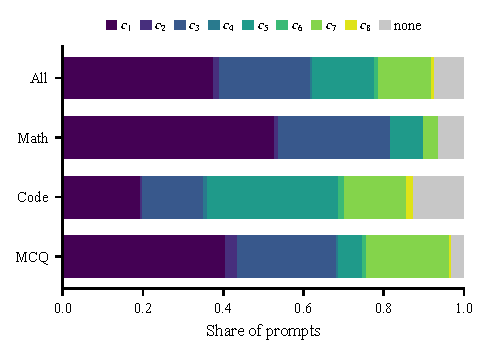
\includegraphics[width=\linewidth]{Figure_1}
\caption{The minimum sufficient cell $\cstar(q)$, in joules, over all prompts
and per family. ``None'' marks prompts that no cell answers.}
\label{fig:cstar}
\end{figure}

Fig.~\ref{fig:cstar} shows where the minimum sufficient cell falls. The
smallest model without thinking is $\cstar(q)$ for 37.5\% of prompts, and the
four non-thinking cells together for 89.2\%. A thinking cell is the cheapest
sufficient choice for 3.6\%, and $c_8$ for 0.75\%. No cell answers 7.25\% of
prompts: 12.5\% of code, 6.25\% of mathematics and 3.0\% of multiple choice.
The families differ in where the rest of the mass lies: on mathematics the
smallest cell suffices for 52.8\% of prompts, while on code the modal
$\cstar(q)$ is 4B without thinking, at 32.8\%.

Counted in tokens, the labels move up the grid. A non-thinking answer is
about as long at 8B as at 0.6B, 223 output tokens against 220, and the token
cost of \eqref{eq:tokcost} has no term for model size, so size is nearly free
and $\cstar(q)$ is $c_7$ for 31.3\% of prompts and $c_5$ for 26.9\%. In
energy an output token costs 0.24\,J at 0.6B and 1.6\,J at 8B. A token count
cannot see that factor of 6.6, and it drives several of the results below.
The attribution of energy within a window does not: apportioning each
window's dynamic energy by token share instead of generation time leaves
$\cstar(q)$ unchanged for 97.3\% of prompts, and per-generation energies
under the two rules have a rank correlation of 0.997.

\subsection{The escalation tax on the local grid}
\label{sec:results-tax}

\begin{table*}[ht]
\centering
\small
\caption{Escalation policies on the local grid over the 1{,}200 gradable
prompts, in joules. Cost per solved divides a policy's mean energy per prompt
by its solved rate, as in \eqref{eq:persolved}. The tax and its two
components are means over servable prompts, and the last column divides the
tax by the mean cost of $\cstar(q)$, 190.6\,J. Imperfect detection is the
illustrative point $p_{\mathrm{acc}} = 0.15$, $p_{\mathrm{rej}} = 0.05$.}
\label{tab:tax}
\begin{tabular}{@{}llrrrrrr@{}}
\toprule
Policy & Detection & Solved (\%) & Cost per solved [95\% CI] & Tax [95\% CI] & Esc. & Stk. & Tax / $c^*$ cost \\
\midrule
P1, frugal climb & oracle & 92.2 & 945.7 [803.2, 1{,}094.5] & 169.4 [139.8, 202.2] & 119.9 & 49.5 & 0.89 \\
P2, think first & oracle & 87.1 & 2{,}970.7 [2{,}634.2, 3{,}326.9] & 1{,}651.7 [1{,}454.7, 1{,}852.6] & 933.3 & 718.4 & 8.66 \\
P3, sticky high & oracle & 79.8 & 3{,}611.7 [3{,}388.3, 3{,}850.8] & 2{,}470.6 [2{,}364.2, 2{,}579.1] & 0.0 & 2{,}470.6 & 12.96 \\
P4, uniform start & oracle & 89.5 & 1{,}763.6 [1{,}603.1, 1{,}930.3] & 915.1 [861.6, 970.9] & 237.8 & 677.3 & 4.80 \\
P4, start skewed to $c_8$ & oracle & 85.3 & 2{,}503.9 [2{,}332.3, 2{,}678.9] & 1{,}581.8 [1{,}511.0, 1{,}653.8] & 135.9 & 1{,}445.9 & 8.30 \\
Random, then $c_8$ & oracle & 84.2 & 2{,}500.8 [2{,}309.9, 2{,}699.4] & 1{,}555.3 [1{,}463.8, 1{,}647.8] & 196.1 & 1{,}359.2 & 8.16 \\
Oracle & oracle & 92.8 & 634.8 [533.2, 741.1] & 0.0 [0.0, 0.0] & 0.0 & 0.0 & 0.00 \\
\midrule
P1, frugal climb & imperfect & 79.9 & 711.5 [613.4, 814.1] & 94.0 [75.1, 113.6] & 93.7 & 0.3 & 0.49 \\
P2, think first & imperfect & 74.9 & 2{,}302.4 [2{,}050.3, 2{,}568.4] & 1{,}093.3 [974.8, 1{,}213.3] & 603.9 & 489.4 & 5.74 \\
P3, sticky high & imperfect & 79.8 & 3{,}611.7 [3{,}388.3, 3{,}850.8] & 2{,}470.6 [2{,}364.2, 2{,}579.1] & 0.0 & 2{,}470.6 & 12.96 \\
P4, uniform start & imperfect & 84.5 & 1{,}659.2 [1{,}524.1, 1{,}799.0] & 877.2 [830.6, 925.6] & 213.5 & 663.7 & 4.60 \\
P4, start skewed to $c_8$ & imperfect & 82.4 & 2{,}468.6 [2{,}308.7, 2{,}633.0] & 1{,}560.1 [1{,}490.7, 1{,}630.4] & 122.0 & 1{,}438.1 & 8.18 \\
Random, then $c_8$ & imperfect & 81.4 & 2{,}440.6 [2{,}262.2, 2{,}626.7] & 1{,}485.9 [1{,}403.3, 1{,}568.8] & 181.1 & 1{,}304.8 & 7.79 \\
\bottomrule
\end{tabular}

\end{table*}

\begin{figure}[ht]
\centering
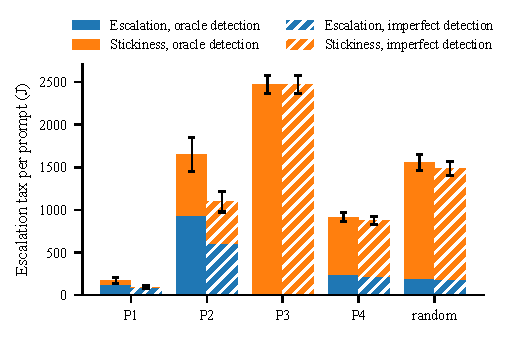
\includegraphics[width=\linewidth]{Figure_2}
\caption{The escalation tax per prompt, in joules, split into escalation and
stickiness, under oracle detection (solid) and imperfect detection (hatched).
Error bars are 95\% bootstrap intervals on the total. P4 starts uniformly
over the cells.}
\label{fig:tax}
\end{figure}

With every failure detected, each policy pays a tax whose interval excludes
zero (Table~\ref{tab:tax}, Fig.~\ref{fig:tax}). The oracle solves the 92.8\%
of prompts that some cell can answer, at 634.8\,J per solved prompt [533.2,
741.1].

Leaving the heaviest cell selected is the most expensive habit. P3 pays a tax
of 2{,}470.6\,J per prompt [2{,}364.2, 2{,}579.1], 12.96 times the cost of
$\cstar(q)$, and all of it is stickiness. It also solves the fewest prompts,
79.8\%, because $c_8$ is not the most accurate cell, and per solved prompt it
pays 3{,}611.7\,J, 5.7 times what the oracle pays. The frugal climb comes
close to the oracle: P1 solves 92.2\% of prompts at 945.7\,J per solved
prompt [803.2, 1{,}094.5], 1.5 times the oracle's figure, and its tax,
169.4\,J [139.8, 202.2] or 0.89 times the cost of $\cstar(q)$, is 71\%
escalation. Its first four rungs are the four cheapest cells, and between
them they are $\cstar(q)$ for 89.2\% of prompts, so the climb meets the
minimum sufficient cell in roughly the order an oracle would rank the cells.
Turning thinking on before moving up a size undoes this: P2 pays 8.66 times
and solves 87.1\%. The population policies fall between the extremes. P4 with
a uniform start pays 4.80 times, three-quarters of it stickiness; with half
of all queries starting at $c_8$ it pays 8.30 times, and random assignment
with recovery at $c_8$ pays 8.16 times. In every family P1 pays the least and
P3 the most.

Detection errors lower the tax and take answers with it. At the illustrative
point, P1's cost per solved prompt falls to 711.5\,J, because a wrong answer
accepted early ends the climb before the expensive rungs, and its solved rate
falls to 79.9\%, below both variants of P4. Every rung is another chance to
accept a wrong answer, so the policies that make the most attempts lose the
most: P1 loses 12.3 points and P2 12.2, while P4 with a uniform start loses
5.0. With no right answers rejected, P1's solved rate falls to P3's once one
wrong answer in five is accepted, 80.2\% against 79.8\%, though it still
spends 680\,J per solved prompt against P3's 3{,}612\,J. Oracle detection is
therefore the regime in which the manual policies answer the most prompts,
not the one in which they spend the least.

The unit changes the ranking. Measured in tokens, P3's tax falls to 4.40
times the cost of $\cstar(q)$ while P2's stays at 8.65, and per solved prompt
P3 spends 2{,}482 tokens against P2's 4{,}719. Tokens charge P2 for every
thinking rung and charge P3 almost nothing for model size, so a token count
ranks sticking with the largest model as the cheaper of the two habits.
Measured energy ranks it as the more expensive, 3{,}611.7\,J per solved
prompt against 2{,}970.7\,J.

\subsection{Routing on the local grid}
\label{sec:results-routing}

\begin{table*}[ht]
\centering
\scriptsize
\caption{Routers on the 243 test prompts, in joules, with a failed routed
answer recovered at $c_8$ and every failure detected. Net cost is the mean
energy per prompt with the router's own energy included; its interval is for
the first training seed, and the standard deviation across three seeds
follows in parentheses. Saving and the change in solved rate are paired
differences against P1, positive when the router is cheaper or solves more,
with Holm-corrected $p$-values. Area is the normalised area under the
router's cost--quality frontier as $\tau$ varies. For the cascade, $\tau$ is
its verification threshold.}
\label{tab:routers}
\setlength{\tabcolsep}{4pt}
\begin{tabular}{@{}lrrrrrrr@{}}
\toprule
Policy or router & $\tau$ & Solved (\%) & Net cost [95\% CI] (s.d.) & Saving vs.\ P1 [95\% CI] & $\Delta$ solved (pp) & $p_{\mathrm{Holm}}$ & Area \\
\midrule
Always $c_8$ & -- & 81.1 & 2{,}676.8 [2{,}430.2, 2{,}926.7] & -- & -- & -- & -- \\
P1, frugal climb & -- & 92.2 & 831.5 [578.2, 1{,}122.1] & -- & -- & -- & -- \\
Random, then $c_8$ & -- & 84.7 & 1{,}896.5 [1{,}633.7, 2{,}170.2] & -- & -- & -- & -- \\
Oracle & -- & 93.0 & 565.5 [377.3, 775.3] & -- & -- & -- & -- \\
\midrule
Direct: TF-IDF + LR & -- & 85.6 & 1{,}521.3 [1{,}249.4, 1{,}803.1] (0.0) & -689.8 [-909.3, -478.8] & -6.6 [-9.9, -3.7] & 0.009 & 0.377 \\
TF-IDF + LR & 0.84 & 88.5 & 1{,}041.0 [801.0, 1{,}304.7] (0.0) & -209.5 [-363.6, -67.7] & -3.7 [-6.2, -1.6] & 0.029 & 0.551 \\
TF-IDF + LR (cost-sens.) & 0.66 & 86.4 & 1{,}162.7 [894.6, 1{,}450.2] (0.0) & -331.2 [-512.7, -164.2] & -5.8 [-8.6, -2.9] & 0.009 & 0.549 \\
Features + LightGBM & 0.76 & 87.7 & 1{,}213.5 [960.1, 1{,}480.7] (102.5) & -382.0 [-562.2, -209.8] & -4.5 [-7.4, -2.1] & 0.009 & 0.479 \\
Features + LightGBM (cost-sens.) & 0.84 & 86.8 & 1{,}209.7 [940.6, 1{,}500.6] (71.2) & -378.2 [-580.8, -191.2] & -5.3 [-8.2, -2.9] & 0.009 & 0.499 \\
Features + XGBoost & 0.84 & 86.8 & 1{,}318.7 [1{,}058.2, 1{,}599.0] (84.1) & -487.2 [-671.6, -315.2] & -5.3 [-8.2, -2.9] & 0.009 & 0.477 \\
Features + XGBoost (cost-sens.) & 0.80 & 87.7 & 1{,}185.2 [919.8, 1{,}469.1] (15.0) & -353.7 [-550.5, -170.3] & -4.5 [-7.4, -2.1] & 0.009 & 0.517 \\
MiniLM + LR & 0.74 & 86.8 & 1{,}156.1 [894.5, 1{,}436.9] (0.0) & -324.6 [-504.6, -161.0] & -5.3 [-8.2, -2.9] & 0.009 & 0.553 \\
MiniLM + LR (cost-sens.) & 0.72 & 87.7 & 1{,}069.8 [821.6, 1{,}339.4] (0.1) & -238.3 [-404.0, -88.9] & -4.5 [-7.4, -2.1] & 0.025 & 0.539 \\
DeBERTa-v3-small & 0.94 & 86.4 & 1{,}491.7 [1{,}218.1, 1{,}786.2] (40.8) & -660.2 [-875.6, -450.8] & -5.8 [-8.6, -2.9] & 0.009 & 0.389 \\
DeBERTa-v3-small (cost-sens.) & 1.00 & 86.4 & 1{,}216.2 [950.5, 1{,}500.9] (128.5) & -384.7 [-567.2, -212.9] & -5.8 [-9.1, -2.9] & 0.009 & 0.433 \\
DistilBERT & 0.92 & 85.6 & 1{,}649.7 [1{,}349.3, 1{,}964.9] (48.4) & -818.2 [-1{,}055.0, -596.6] & -6.6 [-9.9, -3.7] & 0.009 & 0.382 \\
DistilBERT (cost-sens.) & 0.90 & 86.4 & 1{,}130.6 [876.2, 1{,}408.5] (9.7) & -299.1 [-468.5, -143.7] & -5.8 [-9.1, -2.9] & 0.009 & 0.518 \\
Qwen3-0.6B, few-shot & 0.86 & 83.5 & 1{,}872.9 [1{,}583.8, 2{,}168.2] (0.0) & -1{,}041.4 [-1{,}287.8, -797.7] & -8.6 [-12.3, -5.3] & 0.009 & 0.262 \\
Qwen3-0.6B, LoRA & 0.80 & 86.4 & 1{,}262.9 [994.2, 1{,}540.6] (46.8) & -431.4 [-622.1, -248.6] & -5.8 [-9.1, -2.9] & 0.009 & 0.466 \\
Qwen3-0.6B, zero-shot & 0.16 & 84.8 & 1{,}594.6 [1{,}307.2, 1{,}891.4] (0.0) & -763.1 [-998.1, -530.7] & -7.4 [-11.1, -4.1] & 0.009 & 0.366 \\
AutoMix-style cascade & 0.98 & 85.6 & 1{,}587.2 [1{,}305.4, 1{,}880.2] (--) & -755.8 [-971.6, -549.6] & -6.6 [-9.9, -3.7] & 0.009 & 0.355 \\
\bottomrule
\end{tabular}

\end{table*}

\begin{figure}[ht]
\centering
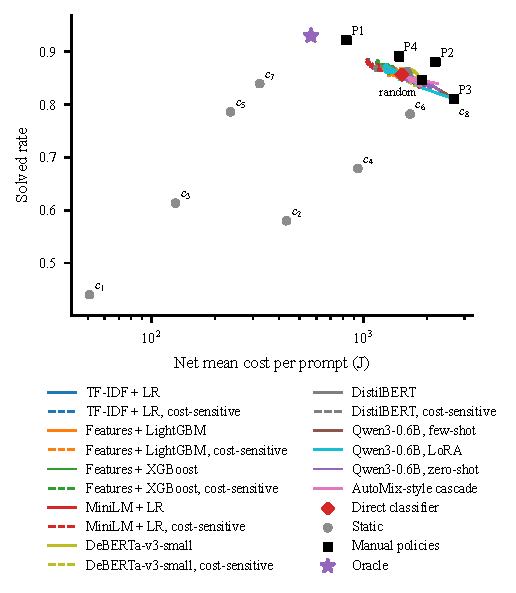
\includegraphics[width=\linewidth]{Figure_3}
\caption{Solved rate against net mean energy per prompt on the test split:
each router as $\tau$ varies (dashed for cost-sensitive training), the
cascade as its threshold varies, the eight cells used alone, the manual
policies and the oracle. Cost is logarithmic.}
\label{fig:frontier}
\end{figure}

Routers were trained on 716 prompts, had $\tau$ chosen on 241 and were
evaluated once on the remaining 243, on which P1 solves 92.2\% at 831.5\,J
per prompt [578.2, 1{,}122.1] and the oracle 93.0\% at 565.5\,J.

Under this recovery rule no router beats the frugal climb, and neither does
the cascade (Table~\ref{tab:routers}); the rule matters, and we return to it
below. The best router,
logistic regression on TF-IDF $n$-grams, solves 88.5\% at 1{,}041.0\,J
[801.0, 1{,}304.7], which is 209.5\,J more than P1 [67.7, 363.6] and 3.7
points fewer [1.6, 6.2]; its net energy per solved prompt is 1.30 times P1's
[1.10, 1.63]. Every other router and the cascade also spends more than P1 and
solves fewer prompts, with Holm-corrected $p \leq 0.03$ in every case. The
shortfall belongs to the routers, not the grid: the oracle spends 32\% less
than P1 [24, 41].

Against the habits that start high, the same router removes most of the tax.
Charged for its own energy, it spends 61\% less than P3 [53, 69] and solves
7.4 points more [4.1, 10.7]; 52\% less than P2 [43, 60]; 45\% less than
random assignment [37, 53]; and 29\% less than P4 with a uniform start [23,
36] at a solved rate within a point of it.

The loss to P1 sits in recovery. A routed answer that fails is resent to
$c_8$, the costliest cell and a less accurate one than $c_7$. The TF-IDF
router guards against that with a high threshold, $\tau = 0.84$: of the test
prompts some cell can answer, it sends 76.1\% to a costlier cell than
$\cstar(q)$ that still succeeds, 9.7\% to a cell that fails and 14.2\%
exactly to $\cstar(q)$, so its tax, 2.70 times the cost of $\cstar(q)$, is
95\% stickiness where P1's is mostly escalation. When a failed routed answer
instead climbs the P1 ladder from the routed cell, the gap closes: every
router then lies within 6\% of P1's energy per solved prompt, solving the
same share of prompts or at most 1.2 points fewer, and four are 2.6\% to
3.4\% cheaper than P1 (Holm-corrected $p = 0.009$).

Imperfect detection reverses the comparison of solved rates. At the
illustrative point P1 solves 80.3\% of prompts, because each of its 1.92
attempts is another chance to accept a wrong answer, while the TF-IDF router
makes 1.18 attempts and solves 87.4\%, which is 7.1 points more [4.2, 9.7],
at 1.76 times P1's energy per solved prompt [1.50, 2.16].

The cascade loses to most routers. It solves 85.6\% at 1{,}587.2\,J per
prompt, and 11 of the 15 one-shot routers are significantly cheaper, the
TF-IDF router by 34\% [23, 45] ($p = 0.002$). Its verification checks are not
the reason, at 9.7\,J each: the check a model runs on its own answer accepts
a wrong one on 33.6\% of the prompts some cell can answer, and each of those
goes to $c_8$ as a misrouted one does, so the cascade makes 2.39 attempts per
prompt, more than any router.

Charging each router for its own energy changes little. No router costs more
than 7.6\,J per decision, 0.6\% of the energy of the queries it routes, and
only three routers change rank between gross and net cost, all within 7\,J of
one another. In tokens the charge matters: the R3 routers pay for their own
prompts, 281 tokens per decision zero-shot and 1{,}141 few-shot, and the LoRA
router falls from fifth to eleventh of 17. The verdict against P1 also
depends on the unit. The TF-IDF router needs 1.35 times P1's latency per
solved prompt [1.13, 1.69] but only 0.76 times its tokens [0.65, 0.89],
because in tokens a failed small attempt costs about as much as an answer
from $c_7$, so P1's climb is dear, while in energy it is nearly free.

Ranked by their best member, the router families keep their order gross and
net. Logistic regression on TF-IDF $n$-grams and on frozen MiniLM embeddings
rank first and second. The fine-tuned encoders approach them only with
cost-sensitive training, which lowered DistilBERT's net cost from
1{,}649.7\,J to 1{,}130.6\,J; it did not help the TF-IDF router. The prompted
R3 routers finish last, beside the cascade: asked for the cheapest sufficient
configuration, the 0.6B model routes low, and the few-shot prompt sends
52.7\% of answerable prompts to a cell that fails. Predicting success per
cell also beats classifying $\cstar(q)$ directly, by 480.3\,J per prompt with
the same TF-IDF features [241.6, 723.8]. The linear routers give the same
result with every training seed, while the gradient-boosted and fine-tuned
ones vary with standard deviations of up to 128.5\,J. Table S4 of the
supplementary material gives each router's overhead per decision.

\subsection{Energy of the reasoning-mode axis}
\label{sec:results-mode}

\begin{figure}[ht]
\centering
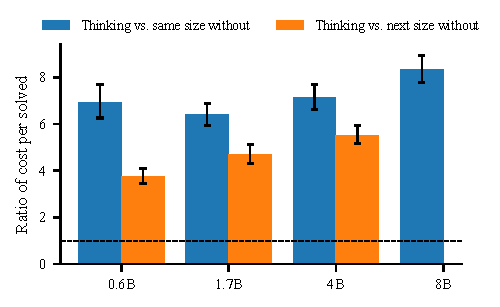
\includegraphics[width=\linewidth]{Figure_4}
\caption{Energy per solved prompt with thinking, relative to the same size
without thinking and to the next size up without thinking. Error bars are
95\% bootstrap intervals, and the dashed line marks parity. 8B has no next
size.}
\label{fig:mode}
\end{figure}

Thinking does not cost a fixed multiple of non-thinking energy
(Fig.~\ref{fig:mode}). Per solved prompt it costs 6.9 times as much as the
same model without thinking at 0.6B, 6.4 times at 1.7B, 7.2 at 4B and 8.3 at
8B, and the intervals at 1.7B, [5.9, 6.9], and 8B, [7.8, 8.9], do not
overlap. The ratio varies more by family than by size: on mathematics it
stays between 4.9 and 6.1, on code it reaches 12.9 at 4B and 15.8 at 8B, and
on multiple choice it peaks at 0.6B, at 15.2, where a non-thinking answer
costs 10\,J.

Under these budgets thinking is also never the cheaper way to buy accuracy on
this grid. Below 8B, the next size up without thinking answers more prompts
than thinking does---59.5\% against 53.0\% at 0.6B, 79.0\% against 65.0\% at
1.7B and 83.6\% against 76.8\% at 4B---and spends 3.8, 4.7 and 5.5 times less
energy per solved prompt, with intervals of [3.5, 4.1], [4.3, 5.1] and [5.1,
6.0]. The same holds in every family, with two exceptions in accuracy: on
code at 0.6B thinking answers 2.8 points more than 1.7B without it, at 4.5
times the energy per solved prompt, and on multiple choice at 4B the two tie.

This conclusion does not wait for the cap reruns. Suppose every capped
thinking generation had been correct, at the energy it used before it was cut
off; thinking would then answer 71.9\%, 84.9\% and 93.0\% of prompts at 0.6B,
1.7B and 4B, more than the next size up at every step, and would still spend
2.8, 3.6 and 4.6 times as much energy per solved prompt. The bound favours
thinking twice over, since an answer that needs a longer budget also needs
more energy. The reruns confirm it: of 219 capped generations rerun with an
8{,}192-token budget, 32.4\% succeed and 27.9\% reach the longer cap as well.
The share rescued rises with size for thinking, from 15.0\% at 0.6B to 52.5\%
at 8B, and the answers it buys are long: a rescued 8B thinking answer has a
median of 5{,}201 output tokens and 8.6\,kJ, against a mean of 362\,J for an
8B non-thinking generation. A rescue moves $\cstar(q)$ for 6.4\% of the rerun
generations and makes 4.6\% of them servable.

Within a size, the premium is one of length. A thinking generation spends
between 0.94 and 1.15 times the energy per output token of a non-thinking
generation at the same size, so output tokens price the mode axis to within
about 15\%, while they miss the factor of 6.6 between sizes.

\subsection{Asymmetry of misallocation}
\label{sec:results-asymmetry}

A router's two errors are priced by sending each servable prompt to the tier
just below its $\cstar(q)$ and to the tier just above, with a failed answer
recovered at $c_8$ as a router's would be. Tiers are the cells in order of
mean energy, $c_1, c_3, c_5, c_7, c_2, c_4, c_6, c_8$, so a step up in energy
is not always a step up in accuracy: the tier above $c_7$ is 0.6B with
thinking. One tier too low fails on 79.8\% of the 663 prompts that have a
lower tier and costs 2{,}625.9\,J more than $\cstar(q)$ [2{,}461.8,
2{,}790.1], 13.8 times its mean cost. One tier too high fails on 24.1\% of
the 1{,}104 prompts that have a higher tier and costs 968.6\,J more [861.4,
1{,}080.8]. Routing too low is therefore 2.71 times as costly [2.43, 3.04] in
energy and 2.85 times [2.55, 3.19] in latency, most on mathematics, at 3.44,
and least on multiple choice, at 1.91.

That is a factor of about three rather than ten, and in tokens the asymmetry
reverses, to 0.86 [0.77, 0.97]. The non-thinking cells lie within 50 tokens
of one another, so their token order has little to do with size: the tier
below $c_3$ is 4B and the tier below $c_5$ is 8B. A step down in tokens then
succeeds on 62\% of prompts, while a step up is often to a thinking cell
whose output is several times as long. In energy and latency, then, a router
should demand more confidence before it routes a prompt down than before it
routes it up, which a threshold $\tau$ above one half does and an argmax over
$\cstar(q)$ does not.

\subsection{Open-ended requests}
\label{sec:results-open}

The open-ended family is reported with the caveat fixed in advance. The local
judge reaches $\kappa = 0.42$ [0.23, 0.59] against the blind human scores,
inside the caveat band, and it is lenient: it passes 65\% of the human
sample, against 57\% for the human rater and 50\% for
\texttt{gpt-5-mini}. The success rates below are therefore those of a lenient
grader; leniency raises every cell's rate, and how it moves $\cstar(q)$
between cells is not known.

On these prompts the grid behaves differently from the gradable families.
Accuracy rises with size and with thinking at every step, from 46.3\% at
$c_1$ to 86.3\% at $c_8$, so here the costliest cell is also the most
accurate, and the cap barely binds: no cell has more than 1.25\% of its
generations reach it. Thinking costs 1.9 to 2.1 times the energy per solved
prompt of the same size without it, against 6.4 to 8.3 on the gradable
families, because a plain open-ended answer is already long and a
generation's tokens only about double with thinking. At 0.6B thinking is
cheaper than the next size up, at 0.62 times the energy per solved prompt of
1.7B without thinking [0.56, 0.71]. A thinking cell is therefore the cheapest
sufficient choice for 22.8\% of open-ended prompts, against 3.6\% of gradable
ones.

The ordering of the policies survives. P1 still pays the least, a tax of 1.46
times the cost of $\cstar(q)$ [1.14, 1.86], and solves 93.8\% of prompts; P3
pays 5.39 times [4.29, 6.85] and solves 86.3\%. The spread is narrower than
on the gradable families because $c_8$ costs 6.5 times the mean cost of
$\cstar(q)$ here rather than 14 times, and is also the most accurate cell. P2
comes close to P1, at 1.79 times, because its second rung, 0.6B with
thinking, is a cheap and useful step on this family. Routing one tier too low
costs 2.03 times as much as one tier too high [1.75, 2.38]. Over all four
families, 1{,}600 prompts, P3 pays 10.59 times the cost of $\cstar(q)$ and P1
1.07 times.

\subsection{The escalation tax on a public benchmark}
\label{sec:results-public}

\begin{table*}[ht]
\centering
\small
\caption{Escalation policies on the public pool under oracle detection, in US
dollars per 1{,}000 queries. P1 climbs the cost--accuracy frontier, P3 uses
its top rung once, P4 starts uniformly over the pool and then climbs, and
Random picks a model uniformly and recovers at the top rung. A policy that
answers fewer queries can show a negative tax, underpaying by failing, so the
tax is read beside the solved column.}
\label{tab:public}
\setlength{\tabcolsep}{4pt}
\begin{tabular}{@{}lrrrrr@{}}
\toprule
Policy & Solved (\%) & Attempts & Cost (\$/1{,}000) [95\% CI] & Tax [95\% CI] & Tax / $c^*$ cost \\
\midrule
P1, climb the frontier & 76.2 & 2.27 & 43.73 [41.98, 45.54] & 16.12 [15.11, 17.17] & 2.69 \\
P3, sticky top & 58.8 & 1.00 & 60.02 [58.62, 61.41] & 47.74 [46.41, 49.04] & 7.96 \\
P4, uniform start & 71.0 & 1.83 & 54.03 [52.34, 55.77] & 28.28 [27.25, 29.29] & 4.72 \\
Random, then top & 64.5 & 1.50 & 47.22 [45.82, 48.61] & 29.48 [28.44, 30.51] & 4.92 \\
\midrule
Always \texttt{deepseek-v3-0324} & 41.3 & 1.00 & 0.76 [0.74, 0.79] & -5.31 [-5.86, -4.78] & -0.89 \\
Always \texttt{qwen3-235b-a22b-2507} & 53.3 & 1.00 & 0.84 [0.81, 0.87] & -5.27 [-5.82, -4.75] & -0.88 \\
Always \texttt{gpt-5} & 57.6 & 1.00 & 29.15 [28.31, 30.01] & 18.34 [17.69, 19.01] & 3.06 \\
Always \texttt{gemini-2.5-pro} & 58.8 & 1.00 & 60.02 [58.62, 61.41] & 47.74 [46.41, 49.04] & 7.96 \\
\midrule
Oracle & 82.0 & 1.00 & 20.88 [19.84, 21.96] & 0.00 [0.00, 0.00] & 0.00 \\
\bottomrule
\end{tabular}

\end{table*}

The public pool spans a factor of 79 in price, from \$0.76 to \$60.02 per
thousand queries, and a factor of 1.6 in accuracy, from 36.9\% to 58.8\%.
Price and accuracy are only loosely related: of the eleven models dearer than
\texttt{qwen3-235b-a22b-2507}, nine answer fewer queries than it does. Only
four of the thirteen lie on the cost--accuracy frontier (Figure~S5 of the
supplementary material), and those four are the ladder a rational escalator
would climb; between them the thirteen answer 82.0\% of the queries. The
distribution of the minimum sufficient model repeats what the local grid
shows: the two cheapest models are the cheapest sufficient choice for 46.5\%
of queries and the costliest model for 2.4\%, while another 29.8\% are
answered most cheaply by a model off the frontier.

Table~\ref{tab:public} gives the policies. Sticky use of the top of the
ladder (P3) pays a tax of 7.96 times the minimum sufficient cost and answers
58.8\% of queries; climbing the frontier (P1) pays 2.69 times, answers 76.2\%
and takes 2.27 attempts per query; the oracle answers 82.0\% at \$20.88 per
thousand. Per solved query the ordering is the same and the comparison is
fair across policies of unequal success: \$25.47 for the oracle, \$57.38 for
P1 and \$102.08 for P3, so a user who always reaches for the strongest model
pays four times what a perfect one-shot router would pay for the same
answers.

Two features of the pool are worth separating from the local grid. First, the
frontier is a subset: a policy climbing it fails on queries only an
off-frontier model answers, and then pays four cheap attempts instead of one
expensive sufficient model. This is why the two cheapest static policies show
a negative tax, and why on SimpleQA even P1 does; they underpay by failing,
which is why cost per solved query carries the comparison. Second, the dollar
tax is larger than the token tax---7.96 against 2.04 for P3---because the
price per token spans two orders of magnitude across providers while the
answers themselves do not differ in length nearly as much. Escalation on a
mixed pool is expensive in a way token counts hide.

The thinking and non-thinking releases of Qwen3-235B-A22B give the public
counterpart of the mode axis. Thinking costs 9.11 times more per solved query
[8.78, 9.47] and, over all nine datasets, answers slightly fewer queries
(52.1\% against 53.3\%). Only 9.3\% of queries need it, so the mode is worth
paying for on a small minority and is picked per query or not at all. Where
reasoning is the point the picture reverses---on GPQA thinking answers 80.3\%
against 58.6\%---which is the same family-dependence the local grid shows.
Scoring a judged Arena-Hard tie as half credit rather than requiring a full
score moves nothing: P3 pays 8.14 times and P1 2.64 times, against 7.96 and
2.69.

\subsection{The escalation tax on a hosted frontier ladder}
\label{sec:results-hosted}

\begin{table*}[ht]
\centering
\small
\caption{Escalation policies on the hosted ladder under oracle detection, in
US dollars per 1{,}000 queries. The static rows are the ladder rungs used
alone. As on the public pool, a policy that answers fewer queries can show a
negative tax by underpaying through failure, so the tax is read beside the
solved column.}
\label{tab:hosted}
\setlength{\tabcolsep}{4pt}
\begin{tabular}{@{}lrrrrr@{}}
\toprule
Policy & Solved (\%) & Attempts & Cost (\$/1{,}000) [95\% CI] & Tax [95\% CI] & Tax / $c^*$ cost \\
\midrule
P1, climb the frontier & 97.1 & 1.38 & 0.34 [0.26, 0.44] & 0.04 [-0.01, 0.09] & 0.22 \\
P2, costly mode first & 97.2 & 1.38 & 0.86 [0.62, 1.14] & 0.26 [0.15, 0.39] & 1.41 \\
P3, sticky top & 92.8 & 1.00 & 1.02 [0.96, 1.09] & 0.80 [0.72, 0.87] & 4.35 \\
P4, uniform start & 95.1 & 1.15 & 1.57 [1.46, 1.69] & 1.27 [1.17, 1.36] & 6.93 \\
Random, then top & 94.6 & 1.12 & 1.61 [1.50, 1.73] & 1.33 [1.22, 1.43] & 7.24 \\
\midrule
Always $h_{1}$ & 74.2 & 1.00 & 0.03 [0.03, 0.03] & -0.15 [-0.23, -0.09] & -0.84 \\
Always $h_{3}$ & 89.5 & 1.00 & 0.18 [0.17, 0.19] & -0.01 [-0.08, 0.05] & -0.04 \\
Always $h_{5}$ & 91.8 & 1.00 & 0.79 [0.74, 0.85] & 0.59 [0.51, 0.65] & 3.20 \\
Always $h_{4}$ & 92.8 & 1.00 & 1.02 [0.96, 1.09] & 0.80 [0.72, 0.87] & 4.35 \\
\midrule
Oracle & 97.5 & 1.00 & 0.25 [0.18, 0.33] & 0.00 [0.00, 0.00] & 0.00 \\
\bottomrule
\end{tabular}

\end{table*}

The six hosted cells, over the 825 prompts every cell answered, span a factor
of 185 in price, from \$0.03 to \$5.77 per thousand queries, and 74.2\% to
92.8\% in accuracy. Four lie on the cost--accuracy frontier (Figure~S6) and form the ladder
$h_1 \rightarrow h_3 \rightarrow h_5 \rightarrow h_4$: \texttt{gpt-5-nano},
then \texttt{gpt-5-mini} at minimal effort, then \texttt{gpt-5} at minimal
effort, then \texttt{gpt-5-mini} at high effort. Both cells left off the
ladder are high-effort ones. \texttt{gpt-5-nano} at high effort costs twice
\texttt{gpt-5-mini} at minimal and answers twelve points fewer, and
\texttt{gpt-5} at high effort, the costliest cell at 5.6 times the price of
\texttt{gpt-5-mini} at high effort, answers slightly fewer queries than it,
91.9\% against 92.8\%. The most expensive thing a user can buy here is not
the most accurate one.

The cheapest cell is the minimum sufficient choice for 74.2\% of queries and
the second rung for another 16.0\%; 2.5\% are answered by no cell, and paid
reasoning effort is the cheapest sufficient choice for 5.1\% across its three
cells. Table~\ref{tab:hosted} gives the policies: P3 pays a tax of 4.35 times
the minimum sufficient cost and answers 92.8\%, P1 pays 0.22 times, answers
97.1\% and takes 1.38 attempts, and the oracle answers 97.5\% at \$0.25 per
thousand. Per solved query P3 pays \$1.10 against the oracle's \$0.25, so
escalation on this ladder is a factor of 4.4 on the price of an answer.
Starting uniformly over the six cells and then climbing (P4) pays 6.93 times,
more than either, because two of its six starting points are cells the
frontier excludes. One static policy is worth naming: \texttt{gpt-5-mini} at
minimal effort used alone costs within noise of the minimum sufficient
cost---a tax of $-0.04$ [$-0.32$, 0.41]---while answering 89.5\% of queries.

The reasoning-effort axis is priced here rather than metered, and the price
is a multiple rather than a margin: high effort costs 11.8, 5.45 and 7.26
times minimal effort at \texttt{gpt-5-nano}, \texttt{gpt-5-mini} and
\texttt{gpt-5}. What it buys shrinks as the model gets stronger. The share of
queries minimal effort fails and high effort answers is 15.2\% at
\texttt{gpt-5-nano}, 6.2\% at \texttt{gpt-5-mini} and 4.1\% at
\texttt{gpt-5}, where overall accuracy moves by a tenth of a point, from
91.8\% to 91.9\%, and falls on multiple choice from 94.9\% to 93.4\%.

The cap does to the hosted cells what it does to the local grid.
\texttt{gpt-5-nano} at high effort spends 1{,}845 reasoning tokens on the
average prompt and hits its 4{,}096-token cap on 18.9\% of them. Counting a
truncated generation as a failure leaves it at 77.8\%; on the responses that
finish it answers 96.0\%, against 74.5\% for the same model at minimal
effort. On code, where its reasoning runs longest, high effort is worse than
minimal outright, 65.3\% against 82.5\%. Reasoning that does not fit the
budget is paid for and discarded, which is the same failure the local 0.6B
and 1.7B thinking cells show.

Because the hosted prompts are the local main subset, each has a $\cstar(q)$
on both ladders, and 765 of the 825 are servable in both; the hosted cells
answer 39 of the 55 prompts the local pool cannot, 24 of them at its two
cheapest rungs, and 16 defeat both. What does not carry across is the rank:
on the prompts both arms answer, the correlation between how far up its own
ladder a prompt must be sent locally and on the hosted ladder is 0.05
($p = 0.16$), so a prompt that needs a large local model is not the one that
needs an expensive hosted tier. The mode axis carries better: the cheap mode
is the cheapest sufficient choice for 96.2\% of the locally servable prompts
and minimal effort for 96.1\% of the hosted ones, and both hold together for
92.8\%. A router trained on one pool therefore transfers its reasoning-mode
decision more readily than its size decision.

\subsection{Carbon of the escalation tax}
\label{sec:results-carbon}

Carbon is energy multiplied by a grid intensity, so a grid rescales every
policy by the same factor and cannot reorder them; what a bracket of
intensities shows is how the choice of policy compares with the choice of
grid. Per 1{,}000 queries, P3's tax is 34\,g of CO$_2$e on a grid at
50\,gCO$_2$e/kWh and 480\,g at 700; P1's is 2.4\,g and 33\,g. Leaving the
largest model selected on a low-carbon grid therefore emits about as much
excess carbon as the frugal climb on a coal-heavy one, the tax differing by a
factor of 14.6 between the two policies where the bracket spans a factor of
14. These are board-level figures for one laptop GPU, and Table S5 of the
supplementary material gives the full bracket.

\section{Discussion}
\label{sec:discussion}

\subsection{Why the effects occur}
\label{sec:why}

\emph{Stickiness is set by the cost distribution.} A policy that never moves
pays the cost of its cell less the cost of $\cstar(q)$, so its relative tax
is the ratio of the two costs less one. All three pools share a shape that
makes that ratio large: the top rung combines the largest model with its
costliest setting, while the mass of $\cstar(q)$ sits at the other end, among
the cheapest one or two options. The tax therefore follows how far the top
rung's price sits above the options that answer most prompts, which is 14
times locally, nine on the public pool and five on the hosted ladder.

\emph{Escalation is small when the ladder's cost order matches the order of
sufficiency.} Each failed rung is paid in full, so a climb is cheap only if
its early rungs are both cheap and likely to succeed. The local P1 ladder has
that property: its first four rungs are the four cheapest cells, and they are
$\cstar(q)$ for 89.2\% of prompts. P2 breaks it at its second rung, where
thinking at 0.6B costs more than any larger non-thinking cell and answers
fewer prompts than any of them. The same property explains the other pools:
the hosted ladder's cheapest cell suffices for three queries in four, while
on the public pool 29.8\% of queries are answered most cheaply by a model the
frontier omits, so the climb cannot stop at $\cstar(q)$.

\emph{The costliest configuration is not the most accurate.} This holds in
every pool we measured on tasks with a checkable answer. Where we can see a
mechanism, it is the generation budget: between 16\% and 20\% of local
thinking generations, and 18.9\% of \texttt{gpt-5-nano}'s at high effort, run
out of tokens before they answer, and a truncated answer fails. A budget is
part of any deployed configuration, so sticky use of the top rung pays twice,
once in cost and again in the answers it loses. Open-ended requests are the
exception: there the cap rarely binds and $c_8$ is the most accurate cell,
yet sticky use of it still pays 5.39 times the minimum sufficient energy.

\emph{Thinking is priced by length, and length varies by family.} Energy per
output token barely moves with the mode, so the mode premium is the ratio of
output lengths, scaled by the change in accuracy. Plain mathematics answers
already write out their working, so thinking lengthens them about five times
and the energy ratio stays between 4.9 and 6.1, while plain code and
multiple-choice answers are shorter, thinking lengthens them 7 to 25 times,
and their ratios reach 15.8 and 15.2. The same accounting shows why a larger
model beats thinking below 8B: a size step keeps the output about as long and
raises energy per generation by 1.4 to 2.7 times, while a mode step keeps the
model and makes the output seven or eight times longer.

\emph{Routing too high is mostly a failure too.} Of the 968.6\,J premium for
routing one tier too high, only 167.5\,J is the higher tier's own excess
cost; the other 801.1\,J is recovery, because a step up in energy order is
not always a step up in accuracy and the step up fails on 24.1\% of prompts.
Against overshoot alone, routing too low would cost 15.7 times as much; the
factor of 2.71 in Section~\ref{sec:results-asymmetry} is lower because the
grid is not monotone, and it also depends on recovering at $c_8$.

\emph{A router loses to the frugal climb in recovery, not in prediction
alone.} P1's failures are cheap because its early rungs are the cheapest
cells. A router's failure is expensive because it recovers at $c_8$, which
costs eight times $c_7$ and answers fewer prompts. A router can avoid that
only by routing high, and the selected threshold does: the best router sends
three answerable prompts in four to a costlier cell than they need, so its
tax is almost all stickiness. Recovering by climbing from the routed cell
brings every router within 6\% of P1. The oracle's 32\% saving over P1
therefore needs a router that is rarely wrong, and the best router we trained
picks $\cstar(q)$ exactly for one prompt in seven.

\emph{Router cost does not separate the families on this grid; training data
does.} Every router's own energy is under 1\% of what it routes, so charging
it leaves the energy ranking almost untouched, and the order comes instead
from how well each family learns from 716 training prompts. A linear model on
$n$-grams or frozen embeddings needs little data, and the fine-tuned encoders
came close to it only when cost-sensitive weights focused training on the
errors that cost most. A 0.6B language model prompted to name the cheapest
sufficient configuration routes low, and on this grid routing low is the
expensive error. Only in tokens, where R3 pays for reading its own prompt,
does charging a router reorder the families. Generating first did not pay for
the cascade either: its checks cost 9.7\,J each, so verification is not what
makes it expensive; the information is weak, since a small model checking its
own answer accepts a wrong one on a third of answerable prompts.

\subsection{Limitations}
\label{sec:limitations}

\emph{The comparator is constructed.} The manual policies of
Table~\ref{tab:policies} are not observed behaviour. We have no logs of how
users of language-model services move between configurations, so the ladders,
the starting distribution of P4 and the detection probabilities are all
assumptions. We limit the damage by reporting a family of policies that
ranges from frugal to wasteful, by quoting headline figures under oracle
detection, in which the manual policies answer the most prompts, and by
sweeping the detection probabilities instead of fixing them. The tax we
report is therefore the tax these policies would pay, not a measurement of
what real users pay, and it is the part of the study that most needs evidence
from outside it. Two of these choices favour the frugal climb, the policy the
routers fail to beat: oracle detection assumes a user who recognises every
wrong answer, which is generous on mathematics and code and implausible on
open-ended work, and the climb makes the most attempts at which such a user
could be fooled, losing 12.3 points at the illustrative detection point.
Model loading is also uncharged, and the climb changes model more often than
any router.

\emph{Attempts are independent single-turn requests, and loading is not
charged.} Each rung is costed by \eqref{eq:policycost} as a fresh request
carrying only the prompt, and succeeds or fails as that cell did during
labelling. A user who escalates within one conversation also resends the
earlier answers, which lengthens every retry, and the stronger configuration
may be helped or misled by seeing a failed attempt; neither effect is
modelled, and the first would make escalation more expensive than we report.
On an 8\,GB GPU that holds one model at a time, a user who escalates across
sizes, or a router that sends consecutive queries to different sizes, also
pays the time and energy of loading a model, which our costs understate most
for whichever policy or router changes size most often.

\emph{Labels come from one sample under fixed caps.} With $k = 1$, each
$s(q, c)$ is a single draw of a stochastic outcome, and $\cstar(q)$ inherits
its noise: on the noise subset a cell's label differs between two samples
8.9\% of the time, and the single-sample $\cstar(q)$ matches the majority of
three for 84.0\% of prompts. The bootstrap resamples prompts with their
labels held fixed, so its intervals do not include that uncertainty. The
labels also depend on the caps. A thinking answer cut off at 4{,}096 tokens
counts as a failure, which is the right rule for deployment but makes
thinking cells look worse than they would with a longer budget. That budget
is below what Qwen3's own guidance suggests for thinking mode, and it
truncates 16 to 20\% of thinking generations, so it shapes three results that
would otherwise read as properties of the models: that $c_8$ answers fewer
prompts than $c_7$, that thinking is never the cheaper way to buy accuracy,
and part of P3's tax. The rerun bounds the effect rather than removing it: a
longer cap moved $\cstar(q)$ for 6.4\% of the capped generations rerun, and
27.9\% of them reached the 8{,}192-token cap too. What the grid shows is how
configurations behave under a deployment budget, not how the models behave
without one.

\emph{Grading is imperfect.} Mathematics answers are compared after
extraction and normalisation, which can reject a correct answer written in an
unusual form; an unparseable multiple-choice answer counts as a failure; and
code is judged by the datasets' own unit tests, which can pass an incorrect
function. The open-ended family depends on a judge that agrees with a human
only moderately, at $\kappa = 0.42$, and passes more answers than either the
human or \texttt{gpt-5-mini}; its results are reported separately and with
that caveat, and every other result covers the gradable families.

\emph{The energy boundary is the GPU board.} NVML reports GPU board power, so
our joules exclude the processor, system memory, storage and display, all of
which draw power while a query is served. Each query's energy is also
apportioned rather than measured, and CPU routers are charged an upper bound
rather than a measurement, which works against R1 in any comparison with a
router measured on the GPU.

\emph{Scope.} Every cell is a Q4\_K\_M quantisation of a Qwen3 model, so size
comparisons are between quantised models; the largest cell has 8B parameters;
thinking is either on or off, although Qwen3 also accepts a budget; and all
measurements come from one laptop and one GPU, so we do not claim the figures
transfer to other hardware. The gradable families come from public
benchmarks, in English and single-turn, which may appear in the models'
training data and are more uniform than live traffic---one reason the corpus
includes an open-ended family. The hosted arm is priced rather than metered,
from one provider's list prices on one date. The comparators are also
simplified: the cascade follows AutoMix without its meta-verifier and climbs
only the P1 ladder, and the prompted R3 routers read their choice from
next-token probabilities without training. Finally, the data are thin for the
comparison between router families---716 training prompts, 243 test prompts
and labels from one sample per cell---so their ranking should be read as what
these families achieve at this scale, not as a general ordering.

\subsection{Implications}
\label{sec:implications}

\emph{Defaults decide most of the tax.} Stickiness is between 74\% and all of
the tax for the policies that often start high, and in all three pools most
prompts are answered by the cheapest options. A service that opens on its
smallest adequate model, with extended reasoning off and a one-step-up
control in view, puts its users on the frugal climb, which spends 1.5 times
the oracle's energy per solved prompt against 5.7 times for leaving the
largest thinking cell selected. Turning reasoning on by default is the harder
choice to defend: within the cap it lost accuracy at 4B and 8B and was never
the cheaper way to buy accuracy on the gradable families, and at
\texttt{gpt-5} high effort answered 4.1\% of queries that minimal effort
missed, at 7.26 times the price, moving overall accuracy by a tenth of a
point. Reasoning is worth paying for on a minority of prompts, which argues
for choosing it per prompt rather than leaving it selected. The default moves
carbon as well as cost.

\emph{A user without a router should change size before mode.} The cheapest
habit on this evidence is to start small with thinking off, move up a size
when an answer fails, and turn thinking on only when the largest size without
it has failed. That advice depends on recognising a wrong answer: a user who
accepts one wrong answer in five keeps the climb's low cost but loses the
extra answers it buys. Prompts the user cannot check are therefore where a
one-shot router has most to offer, since its choice does not depend on their
judgment of the output.

\emph{Cost should be reported in the unit that is paid, per solved prompt.}
Output tokens price the mode axis to within about 15\% but miss the factor of
6.6 in energy per token between 0.6B and 8B, so in tokens P3 looks cheaper
than P2 and routing too low looks cheaper than routing too high, and energy
reverses both; a study that prices a mixed pool in tokens can therefore
favour exactly the misallocations that cost most. The wider pools also show
negative taxes for static policies that underpay by failing, so a tax, like a
cost, means little without the solved rate beside it.

\emph{Deploy a one-shot router against habits, not against a disciplined
climb.} Charged for its own energy, the best router spends 61\% less per
prompt than leaving the 8B thinking cell selected and 29\% less than users
who start at a uniformly random cell, answering more prompts than the first
and about as many as the second. It does not beat a user who climbs sizes
with thinking off and recognises every failure. Two conditions favour it:
when failures are not always recognised it answers 7.1 points more than the
climb, because it makes fewer attempts at which to accept a wrong answer, and
when its failures are recovered by climbing rather than by jumping to the
largest cell it comes within 6\% of the climb's energy. A service that routes
should therefore recover by climbing, and it gains most for users who cannot
check answers.

\section{Conclusion and future work}
\label{sec:conclusion}

A user who tries a configuration, judges the answer and resends the prompt to
a stronger one pays for every attempt, and none of the routing studies we
located measures that cost. We defined it as the escalation tax, split it
into escalation and stickiness, and measured it on three pools: 1{,}200
gradable prompts run through all eight cells of a Qwen3 size-by-mode grid on
a laptop GPU with metered board energy, thirteen public models priced by
their providers, and six hosted cells in which reasoning effort is a paid
setting.

The tax is large, and most of it comes from where a user stays rather than
how they climb. Leaving the 8B thinking cell selected pays 12.96 times the
minimum sufficient energy and answers 79.8\% of prompts, while a frugal climb
pays 0.89 times and answers 92.2\%; the same ordering holds on the public
pool, at 7.96 against 2.69 times, and on the hosted ladder, at 4.35 against
0.22. On the gradable families thinking was never the cheaper way to buy
accuracy: below 8B, the next size up without thinking answered more prompts
for 3.8 to 5.5 times less energy per solved prompt. Open-ended requests,
graded by a judge that agrees with a human only moderately, differed---
thinking cost about twice the energy per solved prompt and the largest
thinking cell was the most accurate---yet the frugal climb still paid the
least tax. Routing one tier too low cost 2.71 times as much energy as routing
one tier too high, an asymmetry that reverses when counted in tokens, as does
the ranking of the two costly habits: cost has to be measured in the unit
that is actually paid.

Whether a router beat the frugal climb turned on the recovery rule. When a
failed route was resent to the 8B thinking cell, the best router, logistic
regression on TF-IDF features, spent 1.30 times the climb's energy per solved
prompt and answered 3.7 points fewer; when failures climbed from the routed
cell instead, every router came within 6\% of it and four were 2.6\% to 3.4\%
cheaper. Against the habits that start high the router spent 64\% less than
leaving the 8B thinking cell selected and 37\% less than a self-verifying
cascade, both per solved prompt, and where users accept 15\% of wrong answers
it answered 7.1 points more than the climb. Charging routers for their own
energy barely changed their ranking, since none cost more than 7.6\,J per
decision. For a user without a router, the evidence points to a short rule:
start small with reasoning off, move up a size before turning reasoning on,
and treat extended reasoning as a choice made per prompt rather than a
setting left on.

Several directions follow. The constructed policies and swept detection
probabilities are the least grounded part of the comparator, and a study that
records how people actually move between the configurations of a tiered
service would replace those assumptions with estimates. Treating the
reasoning budget as a continuous axis rather than a switch would turn the
grid into a surface and the router's decision into a choice of size and
budget; the results make this the most pressing direction, since the cap is a
budget fixed once for every prompt. Because energy per output token barely
changes with the mode within a size while changing by a factor of 6.6 between
sizes, a table of joules per output token per model, measured once, could
turn the token logs services already keep into energy estimates. A router
could also be trained against the recovery rule it will face, since the
threshold that minimises cost when failures jump to $c_8$ is not the one that
minimises it when they climb, or could propose a starting rung for the frugal
climb instead of a final cell. Finally, a cost model in which a retry carries
the conversation so far, and in which changing size pays for loading the new
model, would bring the tax closer to what users of memory-limited hardware
pay.

\section*{CRediT authorship contribution statement}

\textbf{Indrajeet Mondal:} Conceptualization, Methodology, Software,
Validation, Formal analysis, Investigation, Data curation, Writing --
original draft, Writing -- review and editing, Visualization.
\textbf{[Co-author Name]:} [Select the applicable roles, e.g.\
Supervision, Writing -- review and editing, Project administration.]

\section*{Declaration of competing interest}

[Declare any patent application covering the methods reported here, or state
that the authors have no known competing financial interests or personal
relationships that could have appeared to influence this work.]

\section*{Declaration of generative AI and AI-assisted technologies in the
writing process}

[State whether and how generative AI tools were used in preparing this
manuscript, and confirm that the authors reviewed and edited the output and
take full responsibility for the content.]

\section*{Acknowledgements}

[Acknowledge anyone who helped with the research, including help with
language, writing or proof reading, and any funding received, naming the
funding body and grant number.]

\section*{Data availability}

The prompts are drawn from the public benchmark datasets cited in
Section~\ref{sec:setup-labels} and can be reconstructed from them with the
recorded sampling seed and data fingerprints. The generated model outputs,
the per-cell labels and the analysis code are not deposited in a public
repository because they are covered by a pending patent application; they are
available from the corresponding author on reasonable request. The software
used to produce the results is cited as \cite{mondal2026arbiter}.

\section*{Supplementary material}

Supplementary material accompanying this article contains the comparison of
the closest prior systems (Table S1), the full results of validation gates 1
and 2 (Tables S2 and S3), per-decision router overhead (Table S4), the carbon
bracket (Table S5), per-family accuracy of the eight cells (Table S6), the
public pool and hosted cells in cost order (Tables S7 and S8), the detection
sweep and the asymmetry of misallocation (Figures S1 and S2), the token-unit
counterparts of Figures~\ref{fig:tax} and \ref{fig:frontier} (Figures S3 and
S4), and the cost--accuracy frontiers of the two wider pools (Figures S5 and
S6).


{\footnotesize
\setlength{\bibsep}{0pt plus 0.3ex}
\bibliographystyle{elsarticle-num}
\bibliography{refs,refs-methods}}

\end{document}
